%Time-stamp: 'Last modified: 2020-09-15 16:07:32 (d_yasaki)'
\documentclass[ma]{uncgdissertationexp}
% default is 12pt, phd, doublespaced.
% Masters students should use the ma on as shown below.
% \documentclass[ma]{uncgdissertation}
\usepackage{multirow}
\usepackage{microtype, amsmath, amsfonts, amsthm, graphicx, booktabs}
\usepackage[colorlinks=false]{hyperref}
\usepackage[math]{blindtext} 
\usepackage[T1]{fontenc}
\usepackage{lmodern}
\usepackage[english]{babel}
\usepackage{float}
\usepackage{subcaption}
\usepackage{listings}
	\lstset{basicstyle=\ttfamily}
\usepackage{lipsum}
\usepackage{caption}
\usepackage[svgnames]{xcolor}
\usepackage{adjustbox}
\usepackage{multicol}
\usepackage{url}
\usepackage{booktabs}

\chair{Thomas Weighill}
\member{Michael Hull}
\member{Thomas Lewis}   
\member{MEMBER 3}   
\usepackage{graphicx}
\student{Sahil}{Dhawan}  % a full middle name
\title{Analyzing the Topological Properties of 3D STL Files}
\degreeyear{2024}

%% Theorem, Lemma, etc. environments.  You can rename if you wish.                    
% Theorem style and numbering convention                                              
\theoremstyle{plain}
\newtheorem{theorem}{Theorem}[chapter]
\newtheorem{lemma}[theorem]{Lemma}
\newtheorem{proposition}[theorem]{Proposition}
\newtheorem{conjecture}[theorem]{Conjecture}
\newtheorem{corollary}[theorem]{Corollary}
\newtheorem{algorithm}[theorem]{Algorithm}

% Definition type object style and numbering convention                               
\theoremstyle{definition}
\newtheorem{definition}[theorem]{Definition}
\newtheorem{example}[theorem]{Example}

% Remark type object style and numbering                                              
\theoremstyle{remark}
\newtheorem*{remark}{Remark}  % the star makes them not numbered                      
\newtheorem*{notation}{Notation}
\newcommand{\titlecaption}[2]{\caption[#1]{#1. #2}}

%% Other macros
\newcommand{\ZZ}{\mathbb{Z}}  % Integers
\newcommand{\XX}{\mathfrak{X}}  

%% https://tex.stackexchange.com/questions/528129/adding-figure-and-text-in-a-cell-of-a-table
\newcommand*{\tstack}[1]{%
\multicolumn{1}{|c|}{\begingroup        % Add | after the `c` to have vertical lines 
    \renewcommand*{\arraystretch}{1}%
    \begin{tabular}[b]{@{}c@{}}#1\end{tabular}%
  \endgroup
}}
%%------------------------------------------------------------------%%
\pagestyle{plain} % Eliminates running headers 

\begin{document}
\frontmatter      % required
\begin{abstract}
ABSTRACT TEXT
\end{abstract}
\maketitlepage  
\makecopyrightpage
\begin{dedication}
Dedicated to my cats, Piccolo and Gohan, and my dogs, Bebe and Tilly.
\end{dedication}
\makeapprovalpage
\begin{acknowledgments}
It is customary to recognize the assistance of the advisor and/or
committee chair, all other members of the committee, and only those
organizations and/or persons who actually aided the research. If
financial support was provided to make the study possible, credit for
such assistance should be given.
\end{acknowledgments}
\begin{preface}
A preface is a statement that either explains the author's
reasons for pursuing this subject matter or provides a personal
comment about the subject that would not otherwise be included in
the document.
\end{preface}
\tableofcontents
\listoftables
\listoffigures
\mainmatter

\chapter{Introduction}
(2 pages)\\
- what you're doing\\
- tda is ...\\
- related work (FIND NOW), one sentence per paper\\
  - papers that apply tda that relates to cad preferably but other fields are good.\\
  - alpha complex papers\\
    - find some\\
    - homology + meshing\\
  - analysis of 3d shapes\\
    - engineering papers on analyzing cad objects\\
    - manufacturing defects\\
  - meshing 3d shapes\\

\chapter{Background}

\section{Simplicial Homology}

Information in this topic is from \cite{Hatcher_2001}

A simplex is the convex hull of (n+1) points in $\mathbb{R}^{m}$ in general position.
\begin{itemize}
\item 0-simplex: a point
\item 1-simplex: an edge
\item 2-sipmlex: a 'filled-in' triangle, or a triangle containing all points within the boundaries of its edges.
\item 3-simplex: a 'filled-in/solid' tetrahedron, or a tetrahedron containing all points within the boundaries of its 'filled-in' triangles.
\end{itemize}

\section{Persistent Homology}

\subsubsection{Cech Complexes}
$Cech_{r}(X) = \{\sigma \subseteq X \mid \cap_{x \in \sigma} B_{r}(X) \not= \emptyset\}$
\begin{itemize}
\item Balls grow around points of metric space, every time k+1 balls intersect, add a k-dimensional simplex to complex.
\end{itemize}

\subsubsection{Vietoris-Rips Complexes}
$VR_{r}(X) = \{\sigma \subseteq X \mid diam\sigma \leq 2r \}$
\begin{itemize}
\item if subsets of metric space have diameter less than or equal to 2*r, add simplex
\end{itemize}

\subsubsection{Delaunay Complexes}
$Del(X) = \{\sigma \subseteq X \mid \cap_{x \in \sigma} V_{x} \not= \emptyset\}$

$V_{x} = \{y \in \mathbb{R}^{2} \mid ||y-x|| \leq  ||y-z||, z \in X\}$
\begin{itemize}
\item Do not depend on a parameter or intersecting balls (no 'time')
\item Intersecting voronoi cells determine simplices in complex
\end{itemize}

\subsubsection{Alpha Complexes}
$Alpha_{r}(X)=\{\sigma \subseteq X \mid \cap_{x\in \sigma} (B_{r}(X) \cap V_{x}) \not= \emptyset\}$
\begin{itemize}
\item in-between cech and delauney complexes: to construct, take into account both voronoi cell-associated points in metric spce and growing balls around these points
\end{itemize}

\newpage
\section{Background on the STL Filetype}
An STL file is a filetype created for use with 3D files generated by computer-aided design (CAD) programs for 3D printing and other rapid-prototyping applications. STL is ancronym which can be an abbreviation for Stereolithography, Standard Triangle Language, or Standard Tesselation Language. These files are built through triangulation: every set of points creates a triangle which acts as a facet of the object. These triangles are 'filled-in' 2-simplices, and will be fundamental in analyzing the topology of STL files. The information in an STL file can be encoded using binary or in ASCII as a .ast (ASCII STL) file. For our purposes, we will be using .ast files to extract and analyze 3D object data. \cite{STL_info}
\subsection{Converting an .ast File to a Data Structure}
The .ast files are parsed for four strings which are used to denote the beginning and end of the description of facets and vertices: 'facet normal', 'end facet', 'outer loop', and 'end loop', respectively. The data between these strings was then converted into a tuple using python.
\begin{figure}[H]
    \begin{center}
    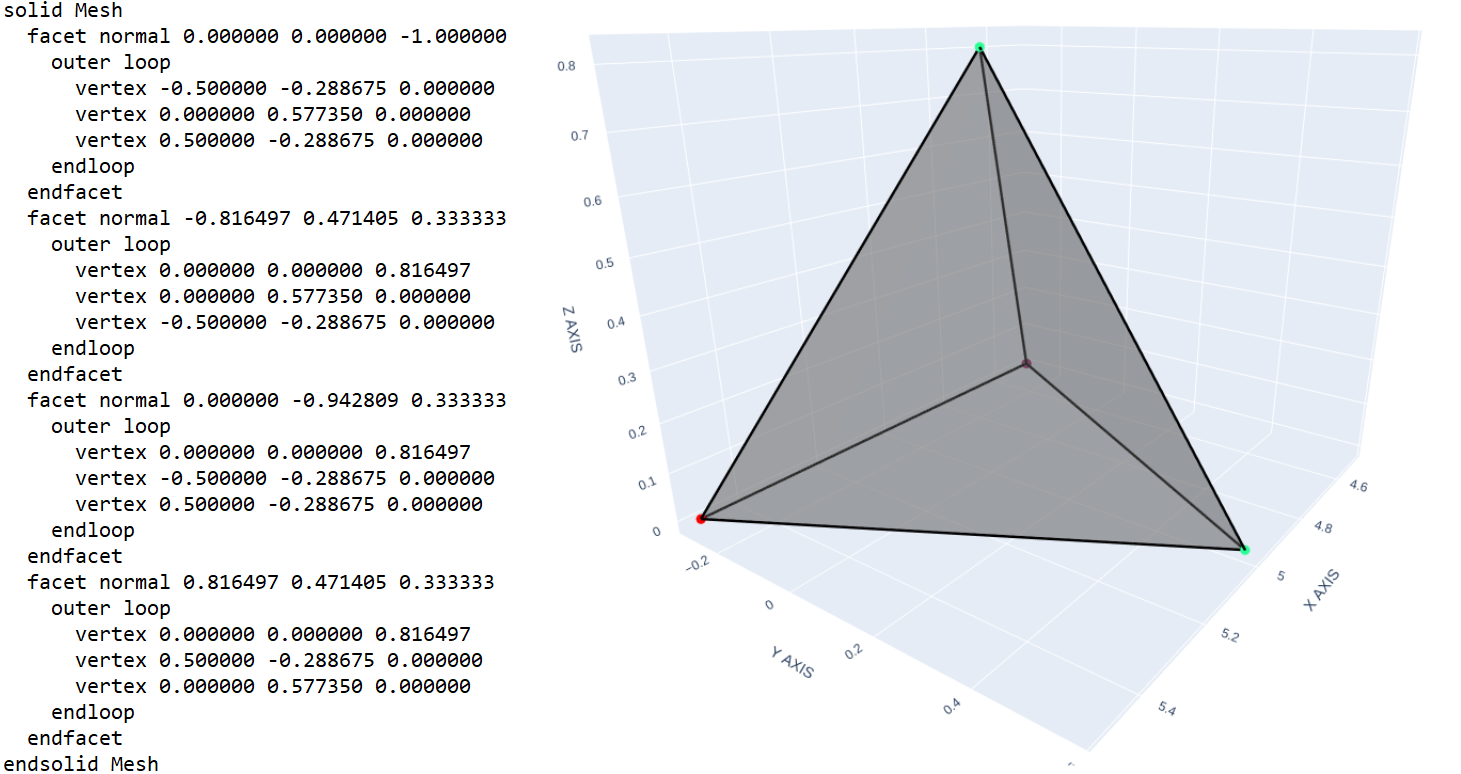
\includegraphics[height=2.9in]{tetrahedron_ast_code_and_plot.png}
    \caption{The contents and 3D plot of an ASCII STL file for a tetrahedron.}
    \label{fig:ast_tetrahedron}
    \end{center}
\end{figure}
\noindent In terms of the contents of an ASCII STL file, a facet should not be confused with a face: a facet must be a triangle, where a face of a polyhedron can be subdivided into multiple facets to achieve triangulation.
\newpage

\chapter{Methods}

\section{Python Libraries}
	\subsection{MeshPy}
	
	\subsection{Gudhi}
\section{Meshing with TetGen}
\subsection{Tetgen Switches}
\cite{tetgen}
\subsubsection{Switch '-p'}
Tetrahedralizes a piecewise linear complex (PLC).

\subsubsection{Switch '-D'}
An option for the \verb"'p'" switch to generate a constrained Delaunay tetrahedralization.

\subsubsection{Switch '-q'}
Refines mesh to improve mesh quality

\subsubsection{Switch '-a'}
Applies a maximum tetrahedron volume constraint on every tetrahedra of the mesh by defining a global constant sizing function.

\section{Filtration Construction with Gudhi}

\section{Persistence Diagram Construction}

\chapter{Results}
\newpage
\section{Cube with Equilateral Triangle Hole}
\begin{table}[H]
	\begin{center}
    \begin{tabular}{|c|c|c|}
    	 \toprule
         \tstack{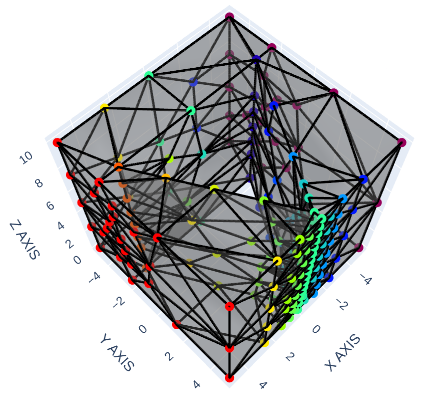
\includegraphics[width=1.75in]{Final Run, (cube - equilateral triangle hole 8 mm) meshpy plotly screenshot.png}\\ {\fontsize{10}{12}\selectfont Equilateral Triangle Hole, 8 mm}} &
         \tstack{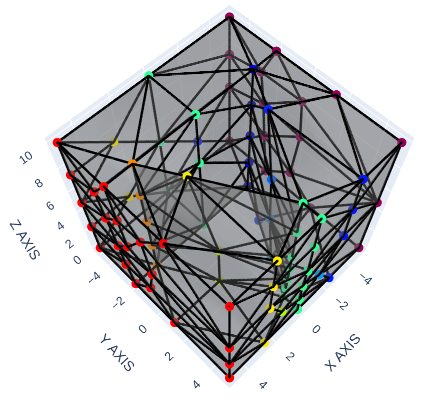
\includegraphics[width=1.75in]{Final Run, (cube - equilateral triangle hole 7 mm) meshpy plotly screenshot.png}\\ {\fontsize{10}{12}\selectfont Equilateral Triangle Hole, 7 mm}} &  
         \tstack{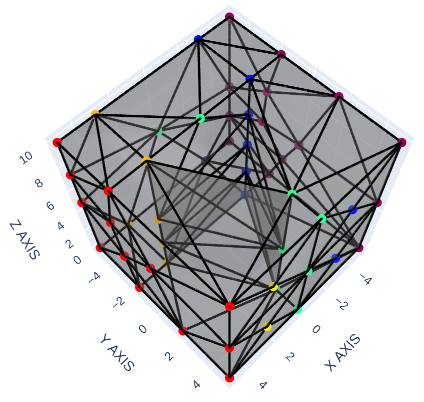
\includegraphics[width=1.75in]{Final Run, (cube - equilateral triangle hole 6 mm) meshpy plotly screenshot.png}\\ {\fontsize{10}{12}\selectfont Equilateral Triangle Hole, 6 mm}} \\
         \midrule
         \tstack{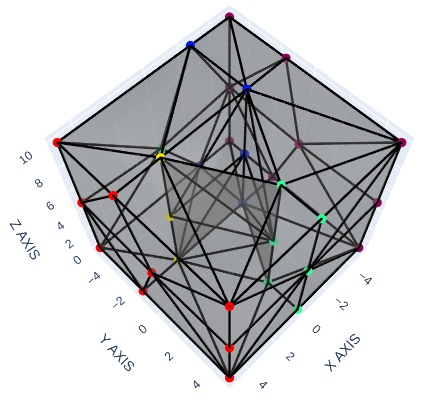
\includegraphics[width=1.75in]{Final Run, (cube - equilateral triangle hole 5 mm) meshpy plotly screenshot.png}\\ {\fontsize{10}{12}\selectfont Equilateral Triangle Hole, 5 mm}} & 
         \tstack{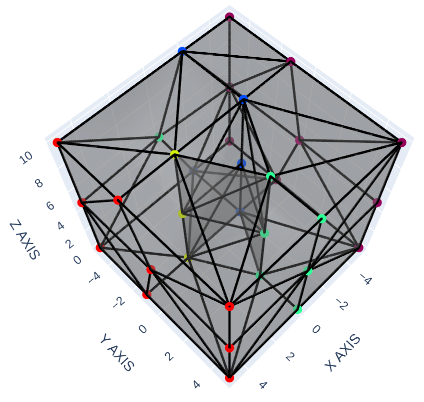
\includegraphics[width=1.75in]{Final Run, (cube - equilateral triangle hole 4 mm) meshpy plotly screenshot.png}\\ {\fontsize{10}{12}\selectfont Equilateral Triangle Hole, 4 mm}} & 
         \tstack{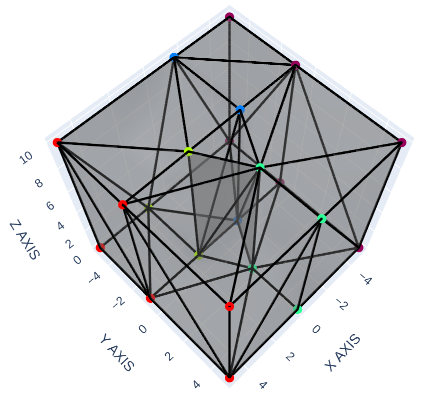
\includegraphics[width=1.75in]{Final Run, (cube - equilateral triangle hole 3 mm) meshpy plotly screenshot.png}\\ {\fontsize{10}{12}\selectfont Equilateral Triangle Hole, 3 mm}} \\
         \midrule
         \tstack{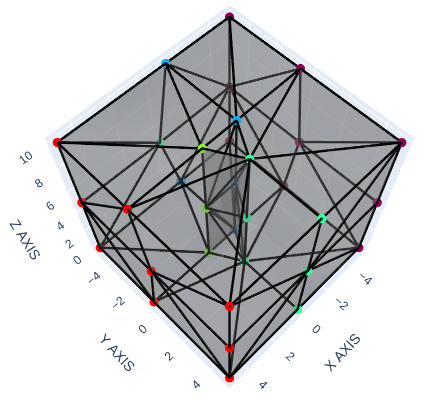
\includegraphics[width=1.75in]{Final Run, (cube - equilateral triangle hole 2 mm) meshpy plotly screenshot.png}\\ {\fontsize{10}{12}\selectfont Equilateral Triangle Hole, 2 mm}} & 
         \tstack{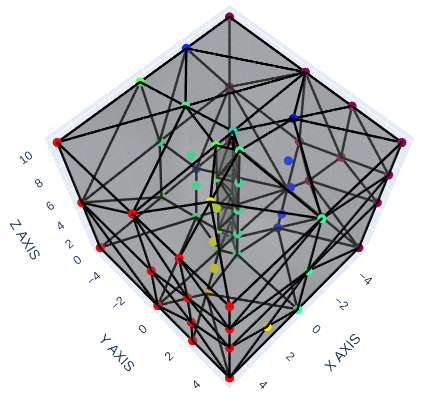
\includegraphics[width=1.75in]{Final Run, (cube - equilateral triangle hole 1 mm) meshpy plotly screenshot.png}\\ {\fontsize{10}{12}\selectfont Equilateral Triangle Hole, 1 mm}} & 
         \tstack{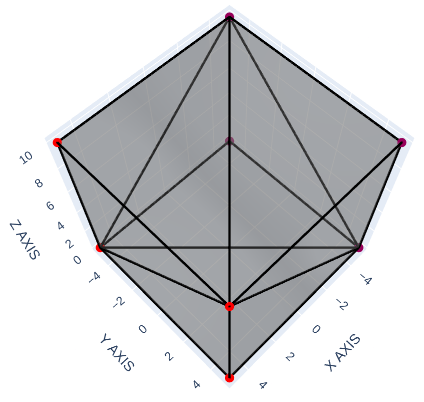
\includegraphics[width=1.75in]{Final Run, (cube - equilateral triangle hole 0 mm) meshpy plotly screenshot.png}\\ {\fontsize{10}{12}\selectfont Equilateral Triangle Hole, 0 mm}} \\
         \bottomrule
    \end{tabular}
    \end{center}
    \caption{MeshPy Plots displayed with Plotly of a cube with an equilateral triangle hole that decreases in size to the original shape.}
    \label{fig:cube_triangle_hole_meshpy_table}
\end{table}

\begin{table}[H]
\begin{center}
    \begin{tabular}{ccc}
         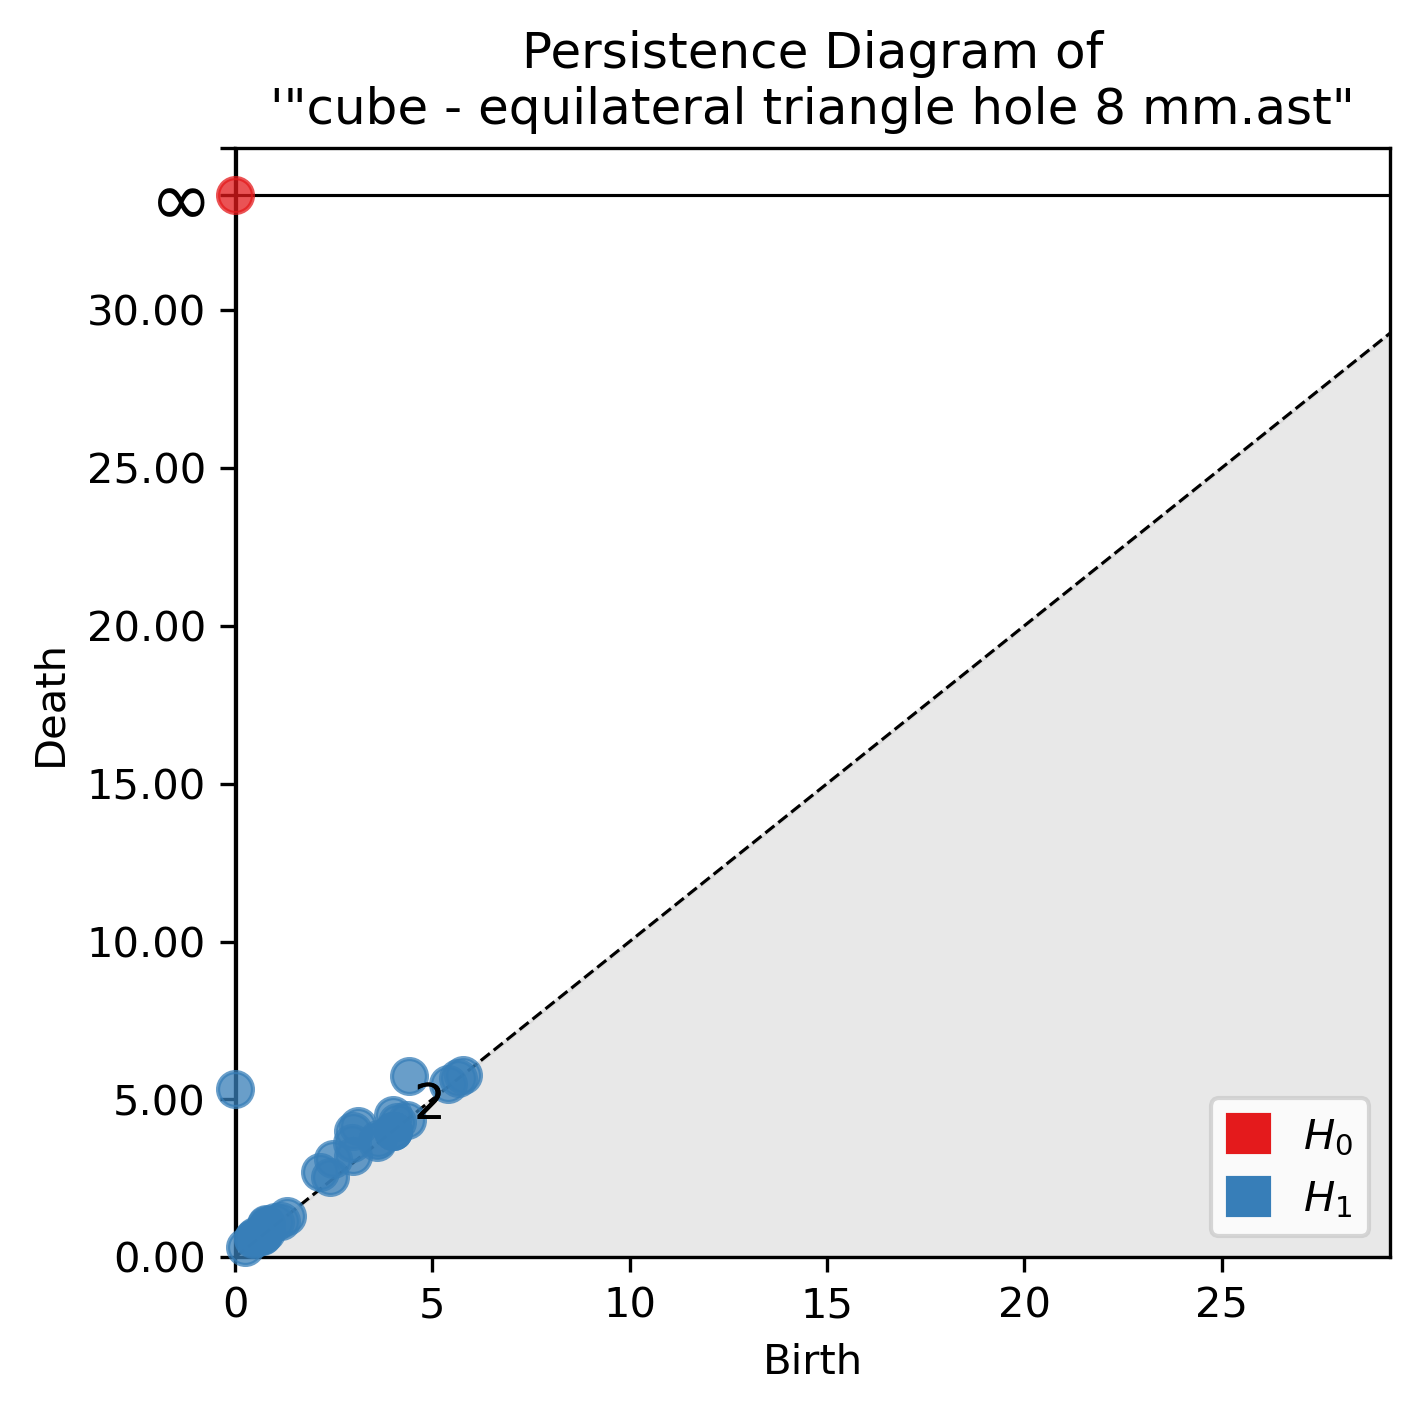
\includegraphics[width=1.875in]{Final Run, (cube - equilateral triangle hole 8 mm) persdia.png} &
         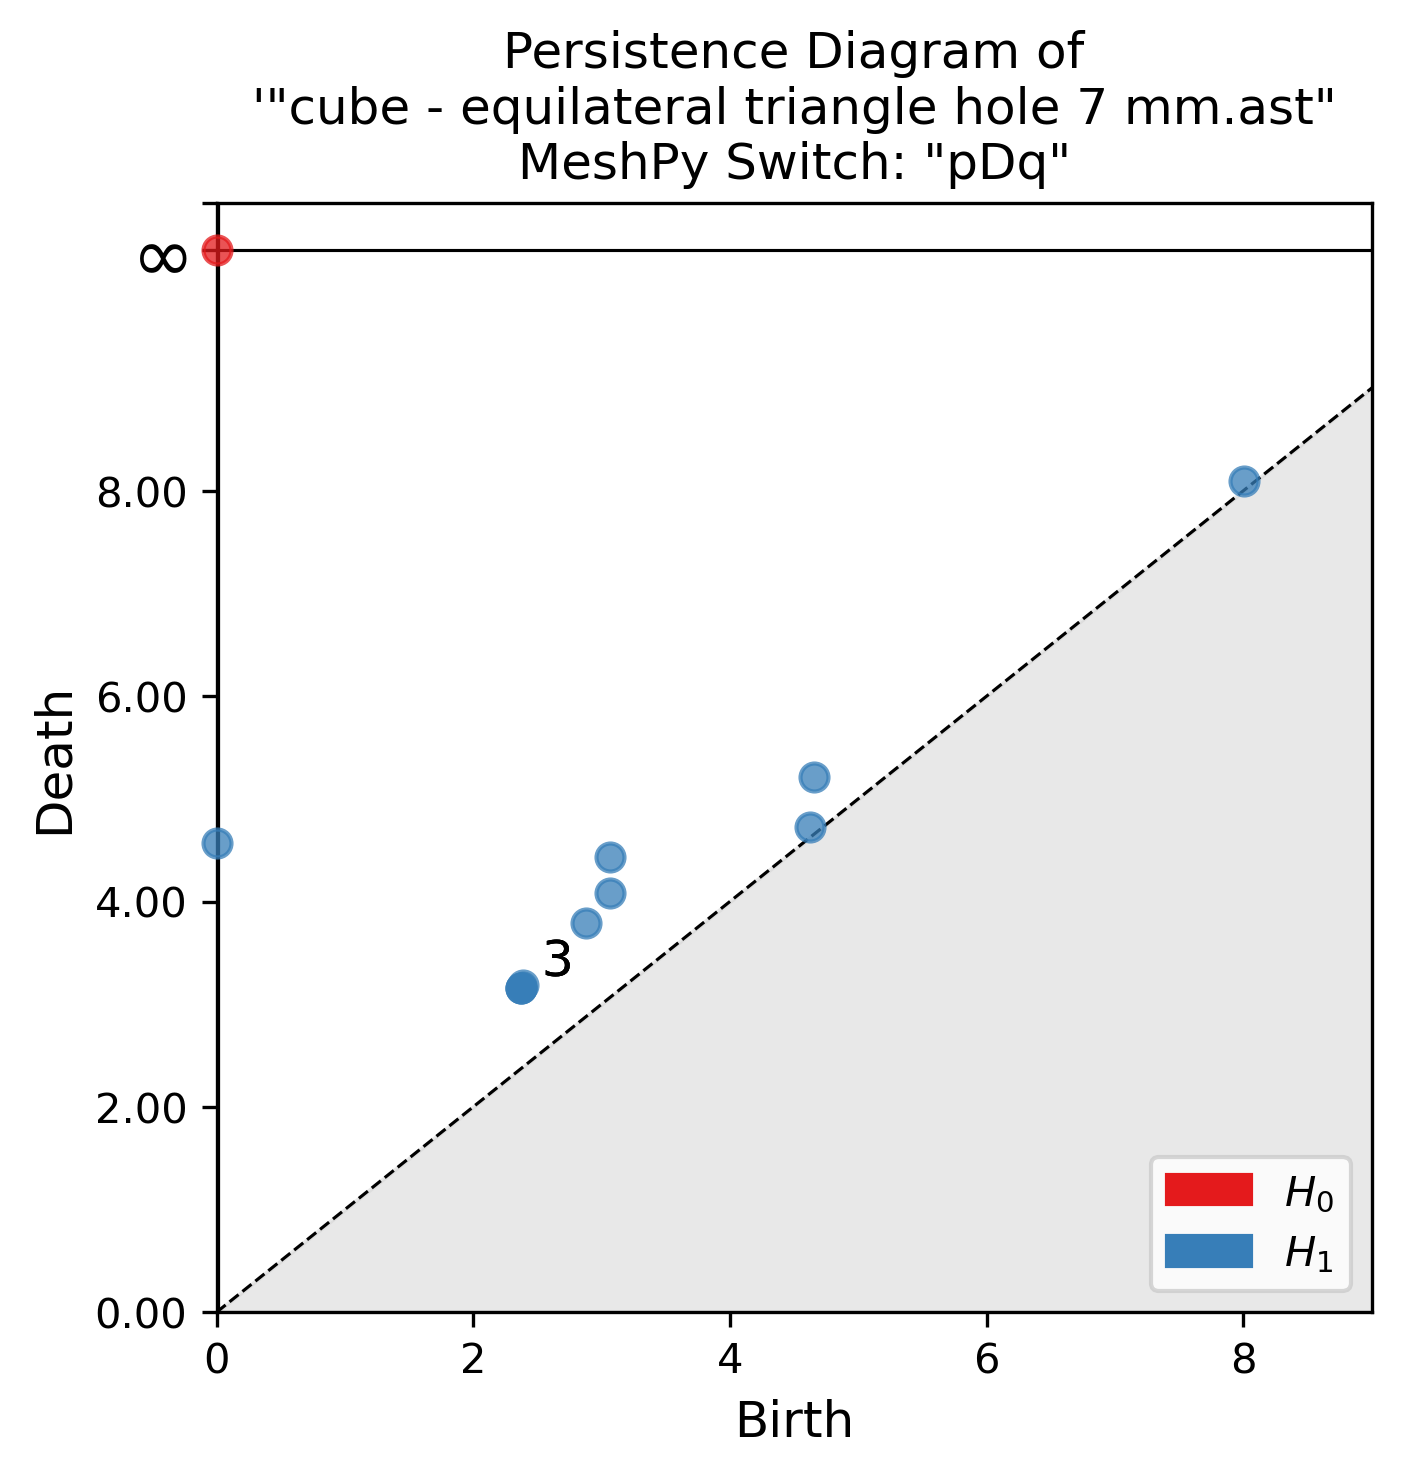
\includegraphics[width=1.875in]{Final Run, (cube - equilateral triangle hole 7 mm) persdia.png} &  
         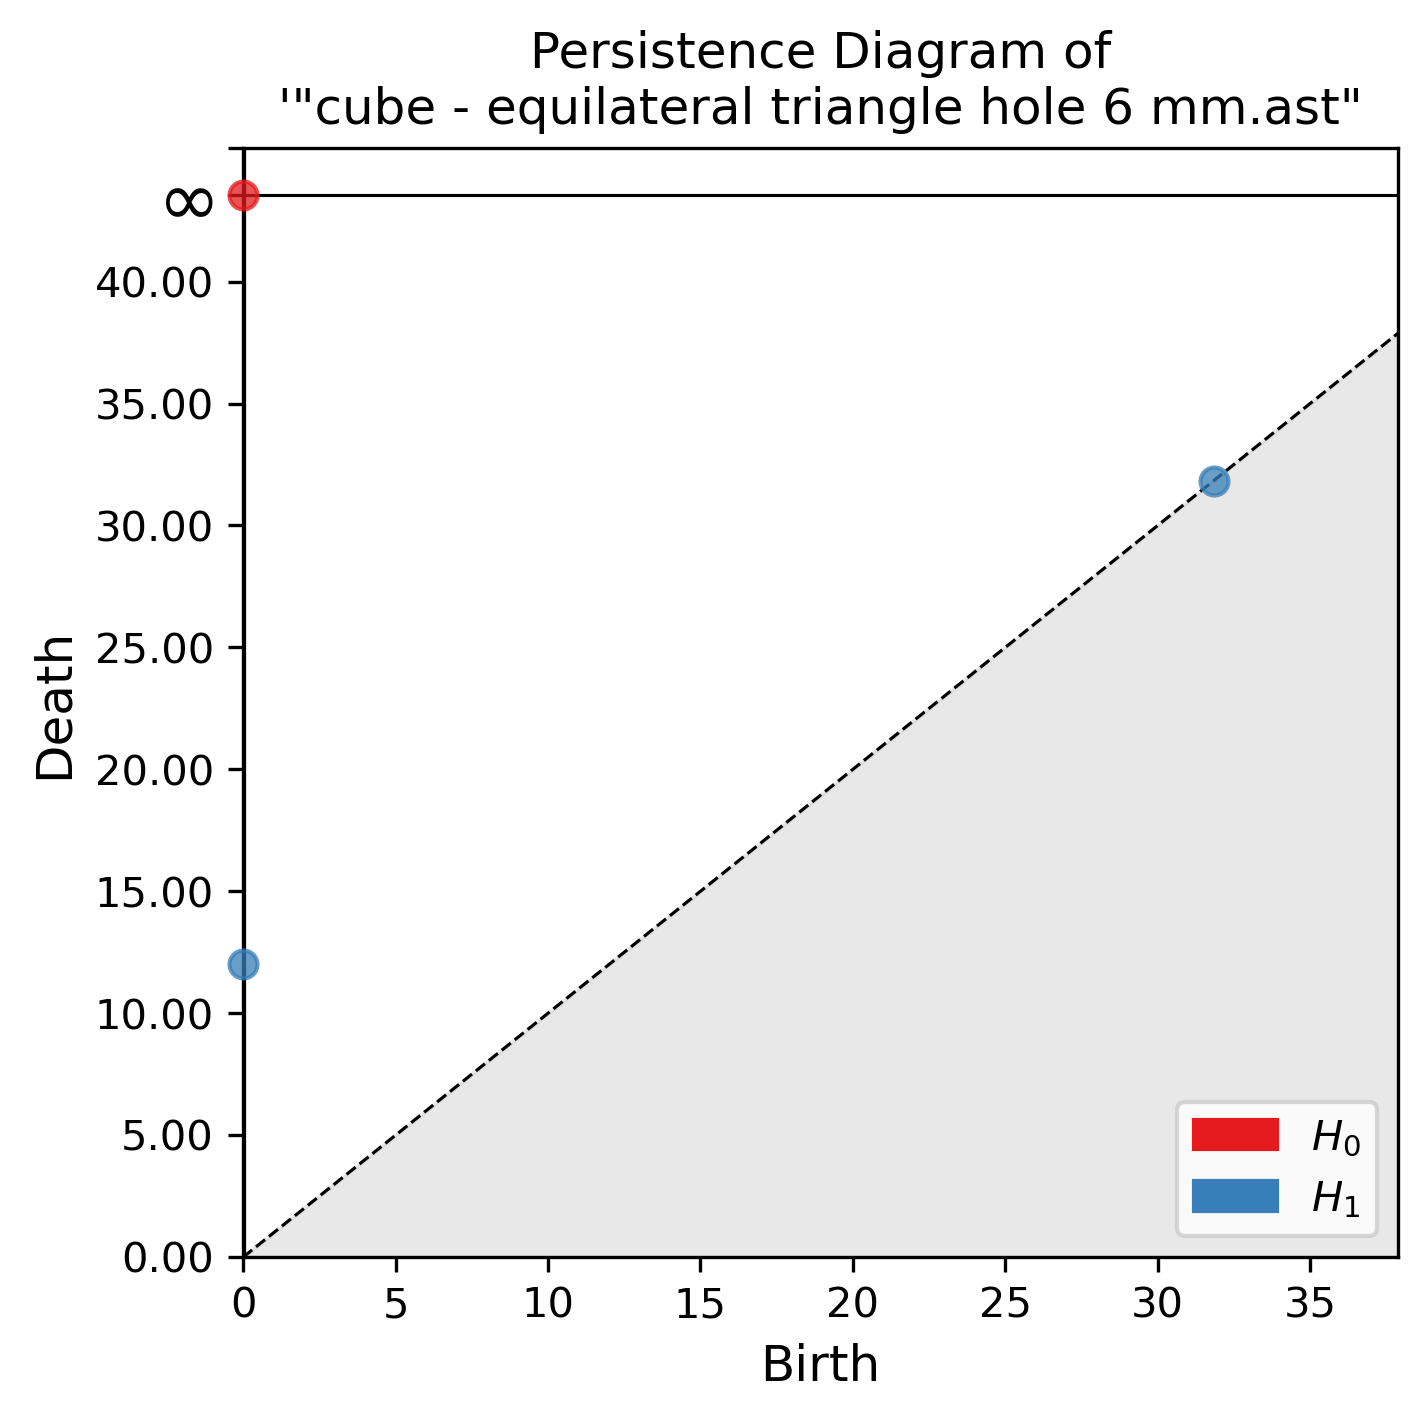
\includegraphics[width=1.875in]{Final Run, (cube - equilateral triangle hole 6 mm) persdia.png} \\
         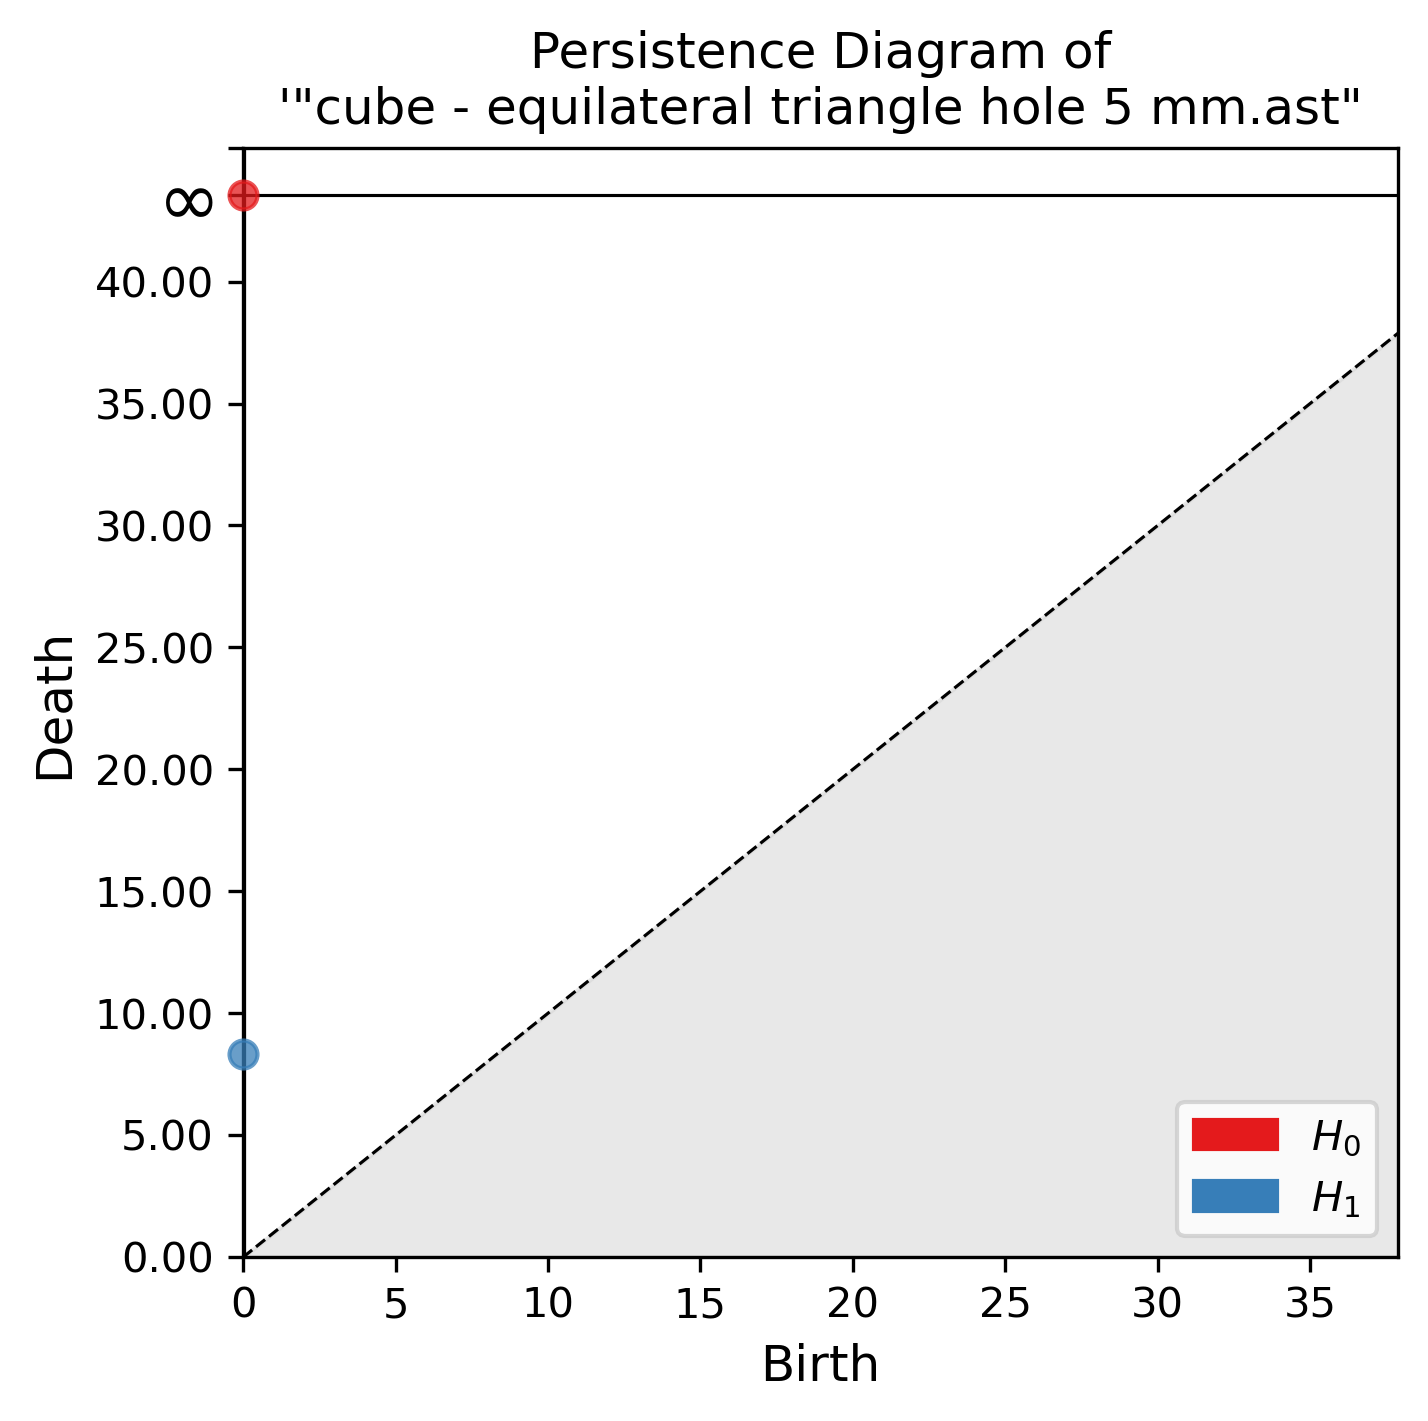
\includegraphics[width=1.875in]{Final Run, (cube - equilateral triangle hole 5 mm) persdia.png} & 
         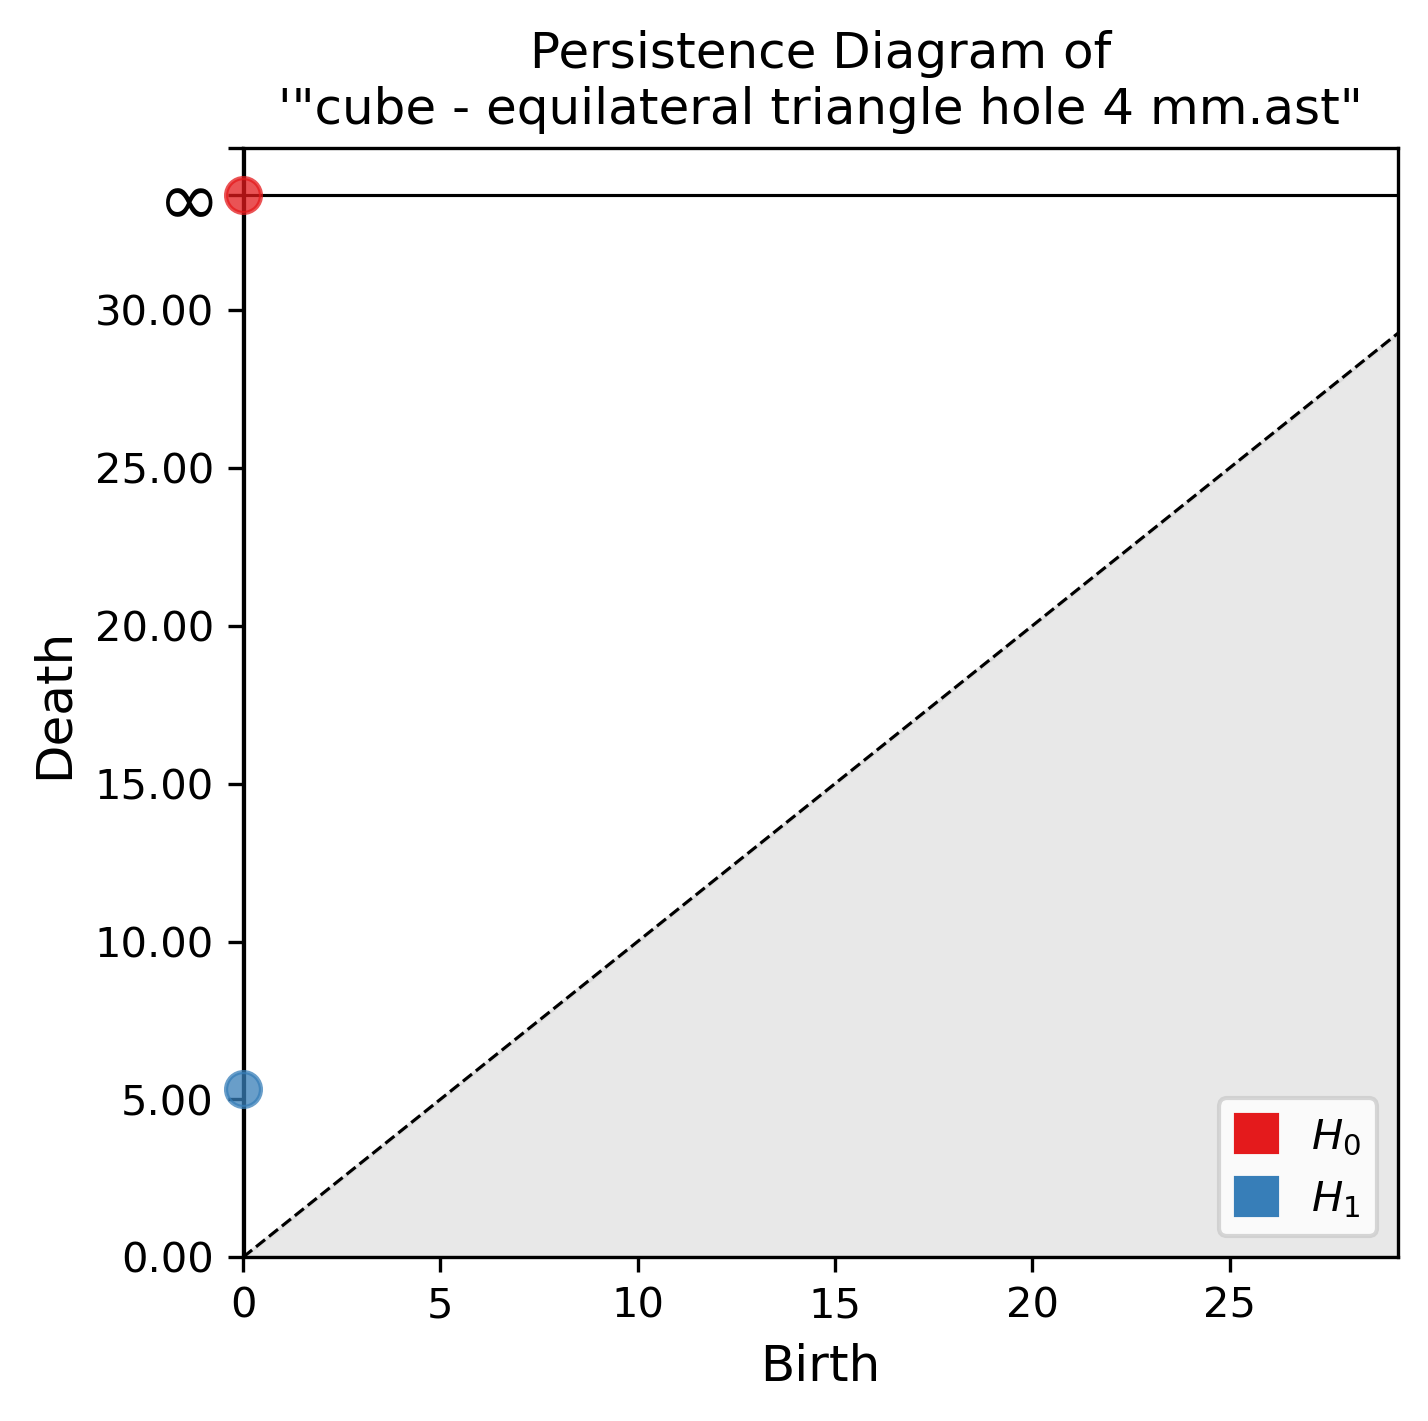
\includegraphics[width=1.875in]{Final Run, (cube - equilateral triangle hole 4 mm) persdia.png} & 
         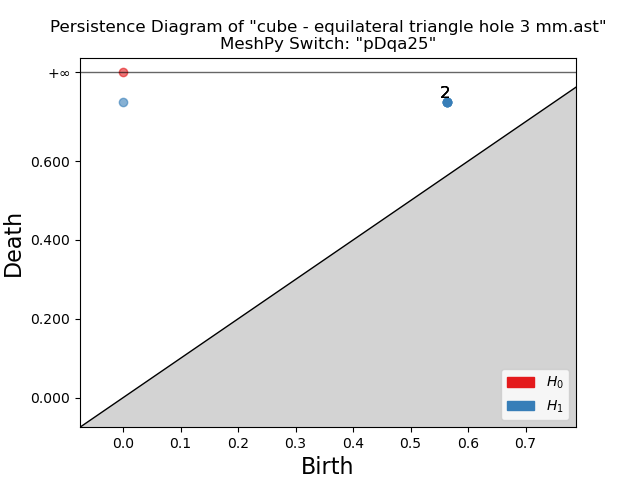
\includegraphics[width=1.875in]{Final Run, (cube - equilateral triangle hole 3 mm) persdia.png} \\
         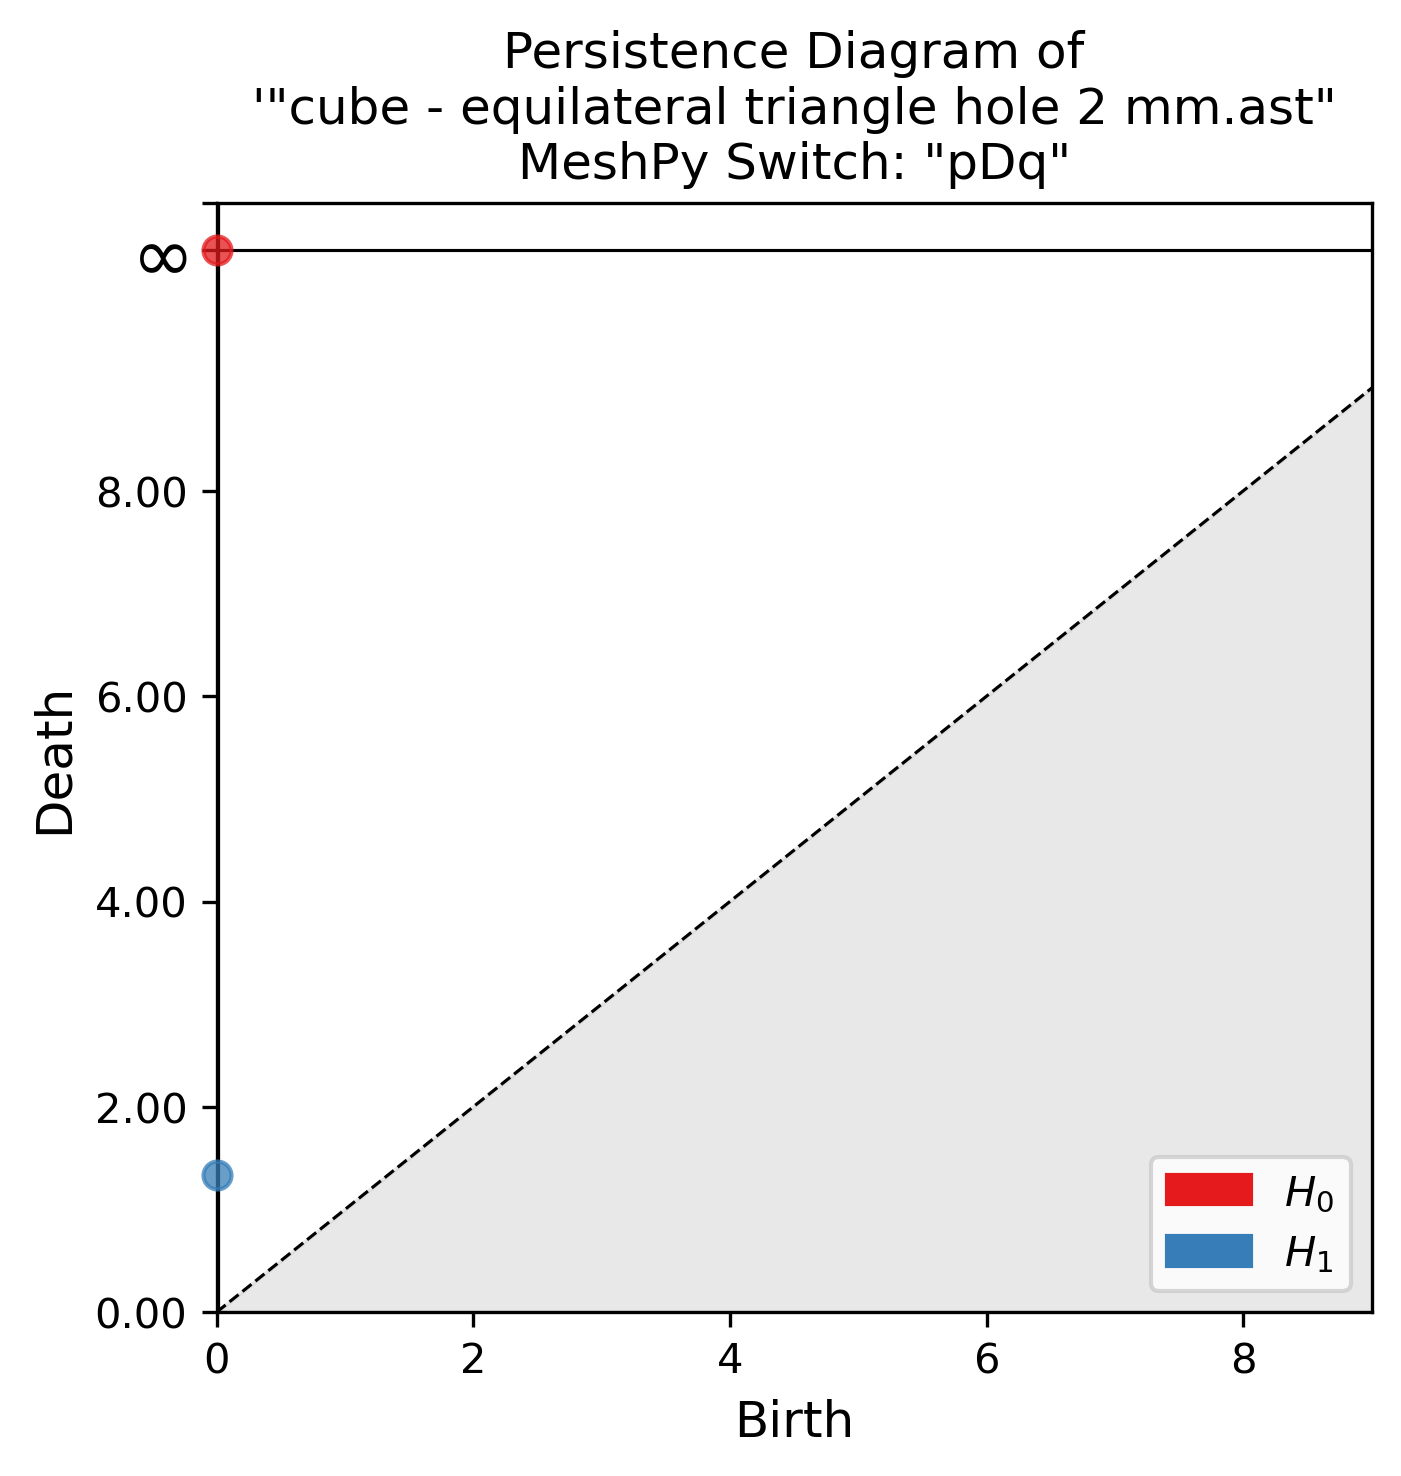
\includegraphics[width=1.875in]{Final Run, (cube - equilateral triangle hole 2 mm) persdia.png} & 
         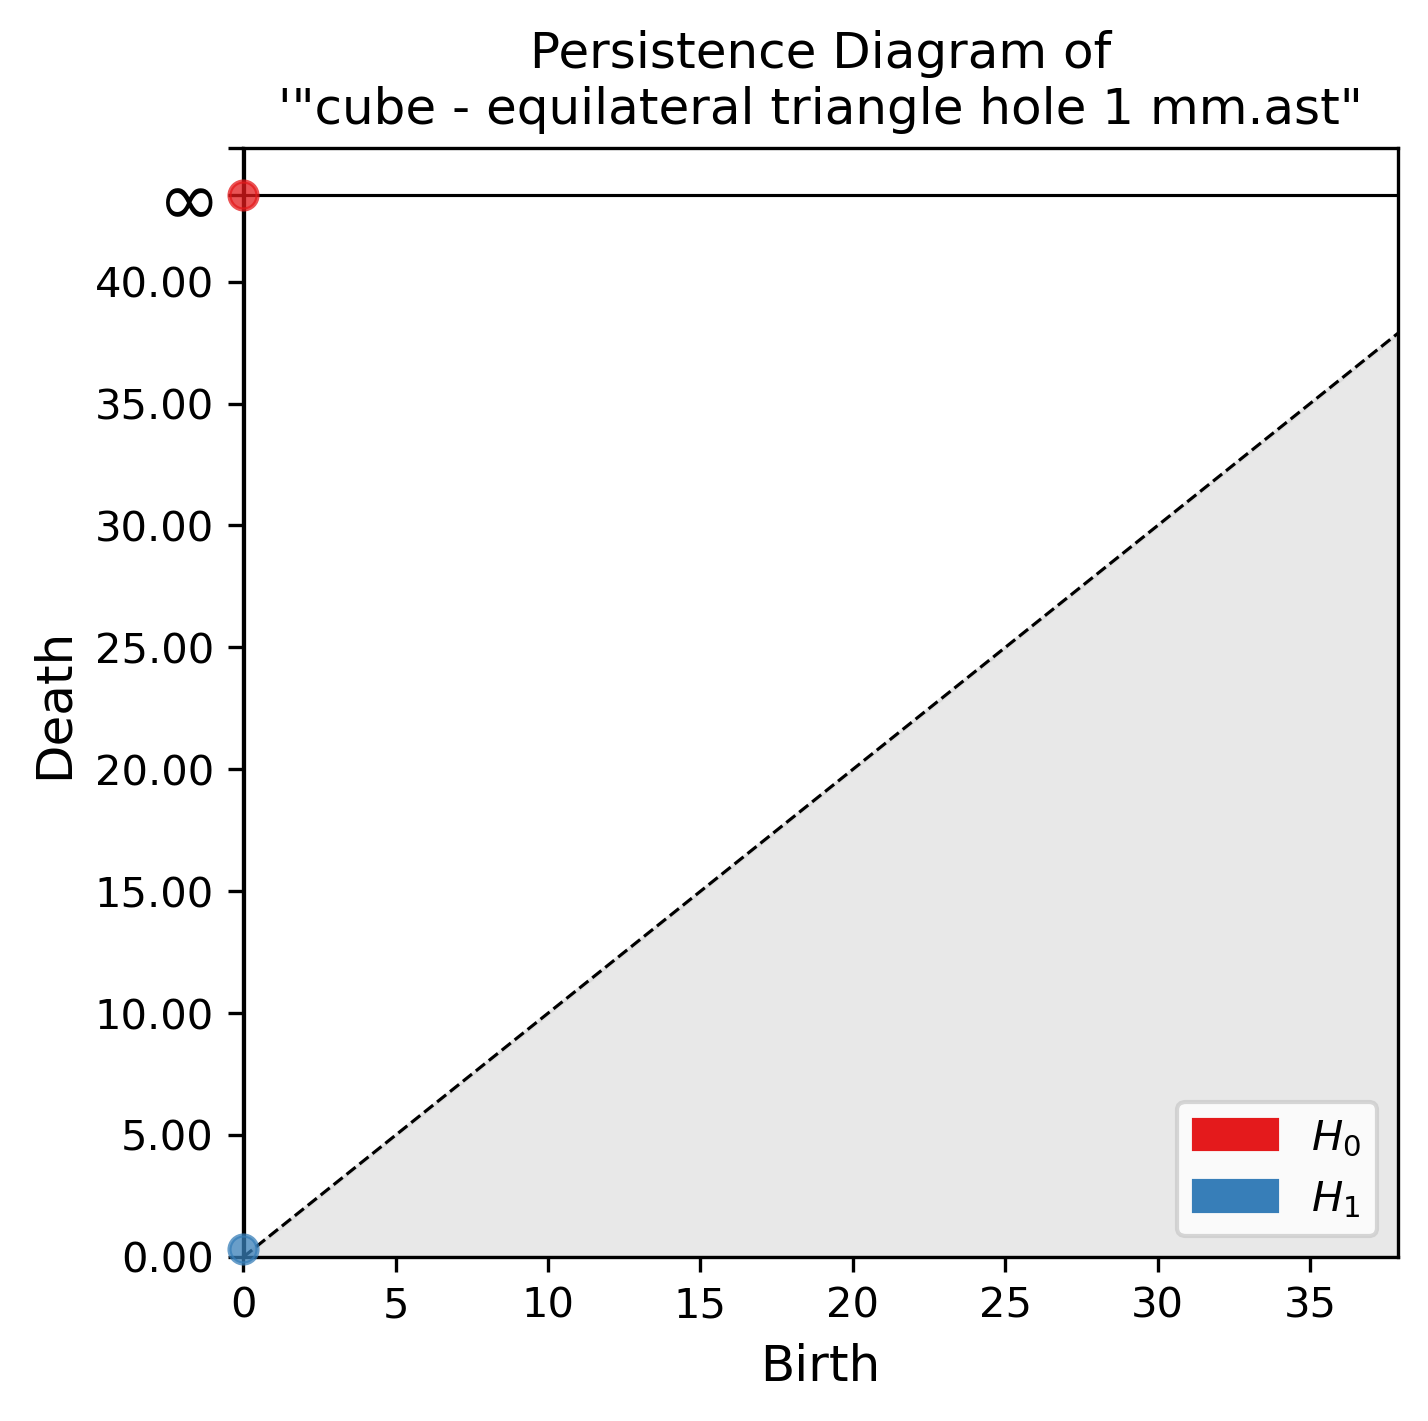
\includegraphics[width=1.875in]{Final Run, (cube - equilateral triangle hole 1 mm) persdia.png} & 
         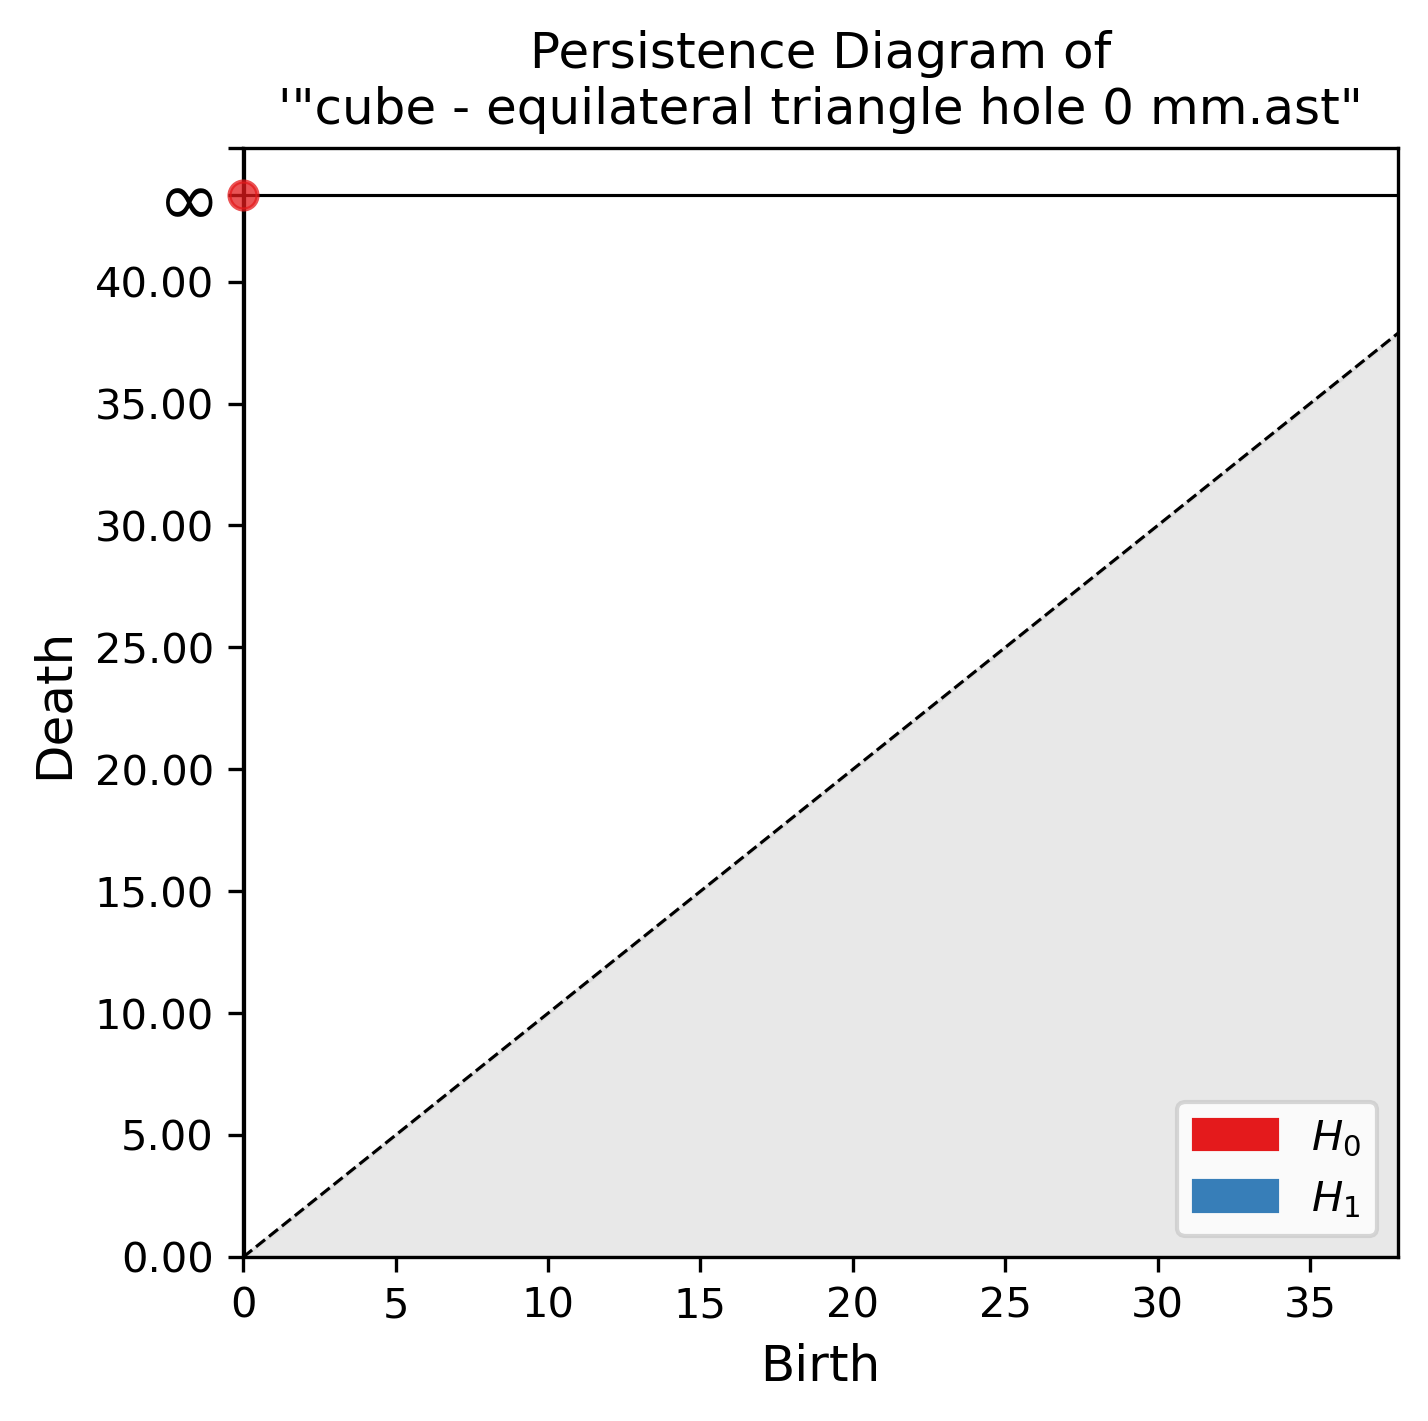
\includegraphics[width=1.875in]{Final Run, (cube - equilateral triangle hole 0 mm) persdia.png} \\
    \end{tabular}
    \end{center}
    \caption{Persistence Diagrams of a cube with an equilateral triangle hole that decreases in size to the original shape.}
    \label{fig:cube_triangle_hole_persdia_table}
\end{table}

\section{Rectangular Prism Ring with Cut}
\begin{table}[H]
\begin{center}
    \begin{tabular}{cccc}
    \toprule
         \tstack{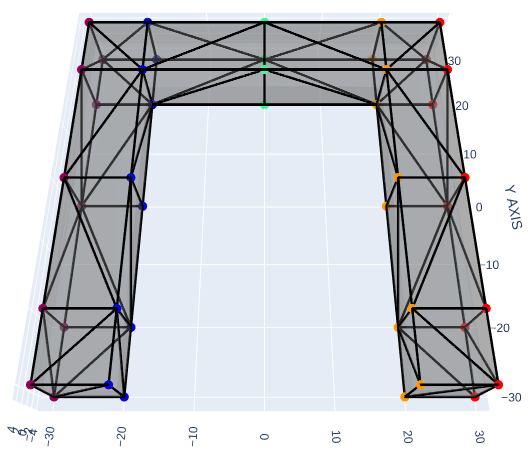
\includegraphics[width=1.4in]{Final Run, (rect prism ring 40 mm cut) meshpy plotly screenshot.png}\\ {\fontsize{10}{12}\selectfont 40 mm cut}} &
         \tstack{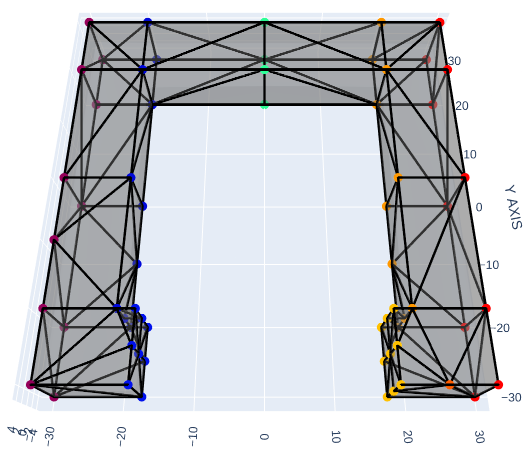
\includegraphics[width=1.4in]{Final Run, (rect prism ring 35 mm cut) meshpy plotly screenshot.png}\\ {\fontsize{10}{12}\selectfont 35 mm cut}} &
         \tstack{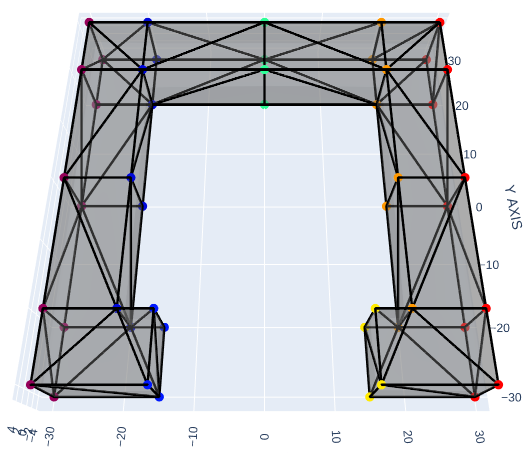
\includegraphics[width=1.4in]{Final Run, (rect prism ring 30 mm cut) meshpy plotly screenshot.png}\\ {\fontsize{10}{12}\selectfont 30 mm cut}} &
         \tstack{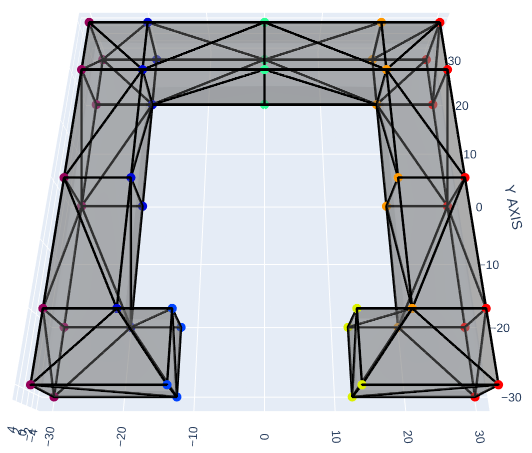
\includegraphics[width=1.4in]{Final Run, (rect prism ring 25 mm cut) meshpy plotly screenshot.png}\\ {\fontsize{10}{12}\selectfont 25 mm cut}} \\ 
    \midrule
         \tstack{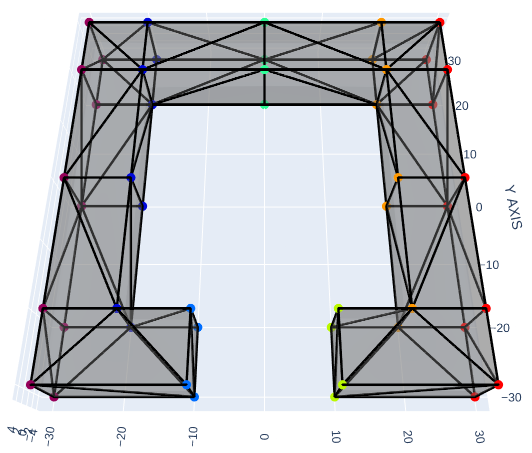
\includegraphics[width=1.4in]{Final Run, (rect prism ring 20 mm cut) meshpy plotly screenshot.png}\\ {\fontsize{10}{12}\selectfont 20 mm cut}} & 
         \tstack{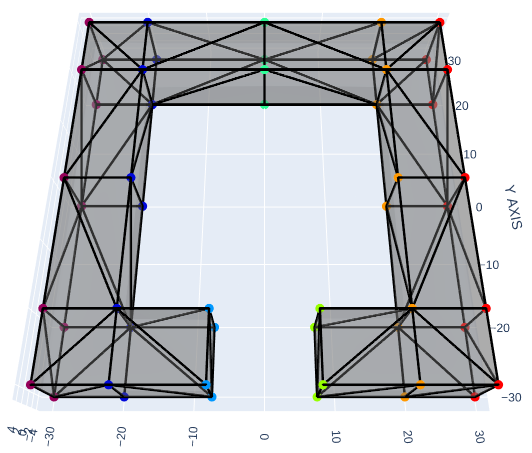
\includegraphics[width=1.4in]{Final Run, (rect prism ring 15 mm cut) meshpy plotly screenshot.png}\\ {\fontsize{10}{12}\selectfont 15 mm cut}} &
         \tstack{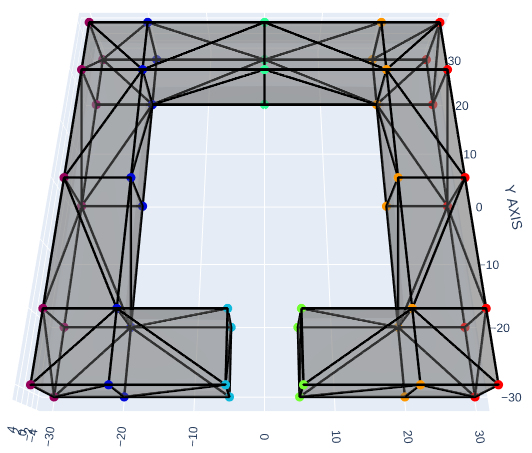
\includegraphics[width=1.4in]{Final Run, (rect prism ring 10 mm cut) meshpy plotly screenshot.png}\\ {\fontsize{10}{12}\selectfont 10 mm cut}} & 
         \tstack{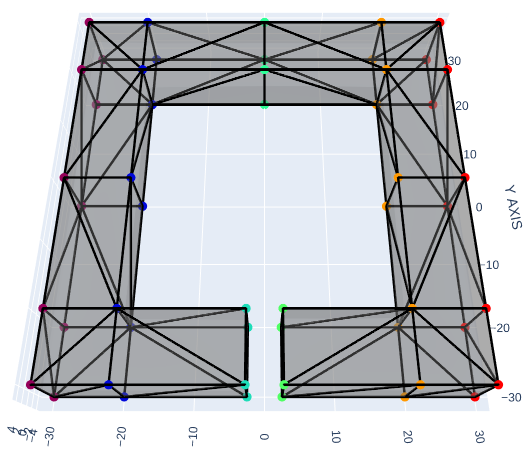
\includegraphics[width=1.4in]{Final Run, (rect prism ring 05 mm cut) meshpy plotly screenshot.png}\\ {\fontsize{10}{12}\selectfont 05 mm cut}} \\ 
    \midrule
         \tstack{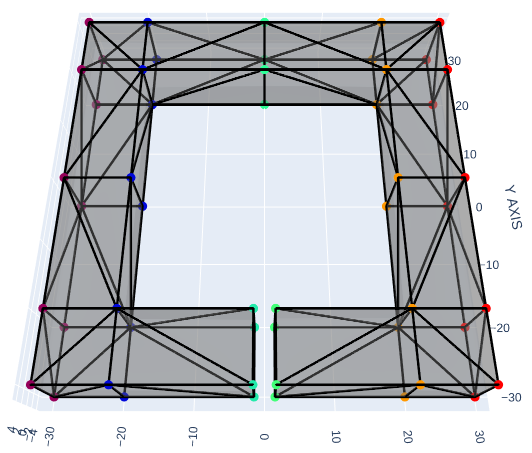
\includegraphics[width=1.4in]{Final Run, (rect prism ring 03 mm cut) meshpy plotly screenshot.png}\\ {\fontsize{10}{12}\selectfont 03 mm cut}} &
         \tstack{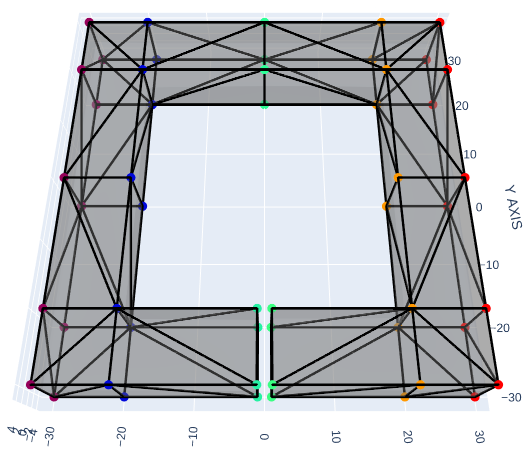
\includegraphics[width=1.4in]{Final Run, (rect prism ring 02 mm cut) meshpy plotly screenshot.png}\\ {\fontsize{10}{12}\selectfont 02 mm cut}} &
         \tstack{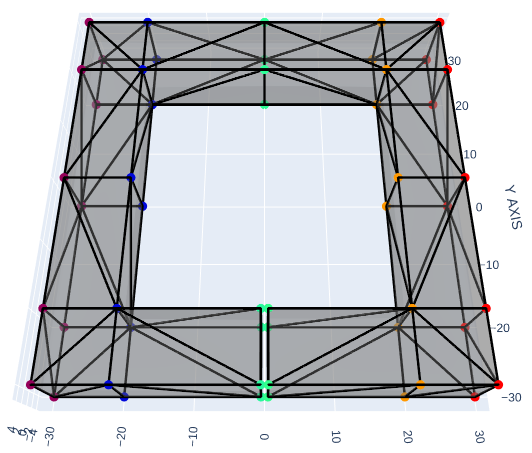
\includegraphics[width=1.4in]{Final Run, (rect prism ring 01 mm cut) meshpy plotly screenshot.png}\\ {\fontsize{10}{12}\selectfont 01 mm cut}} &
         \tstack{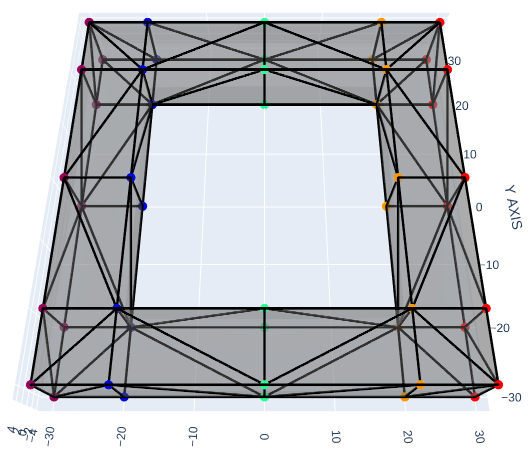
\includegraphics[width=1.4in]{Final Run, (rect prism ring 00 mm cut) meshpy plotly screenshot.png}\\ {\fontsize{10}{12}\selectfont 00 mm cut}} \\
    \bottomrule
    \end{tabular}
    \end{center}
    \caption{MeshPy Plots displayed with Plotly of a rectangular prism ring with a cut that decreases to the original shape.}
    \label{fig:rect_prism_ring_meshpy_table}
\end{table}

\begin{table}[H]
\begin{center}
    \begin{tabular}{ccc}
         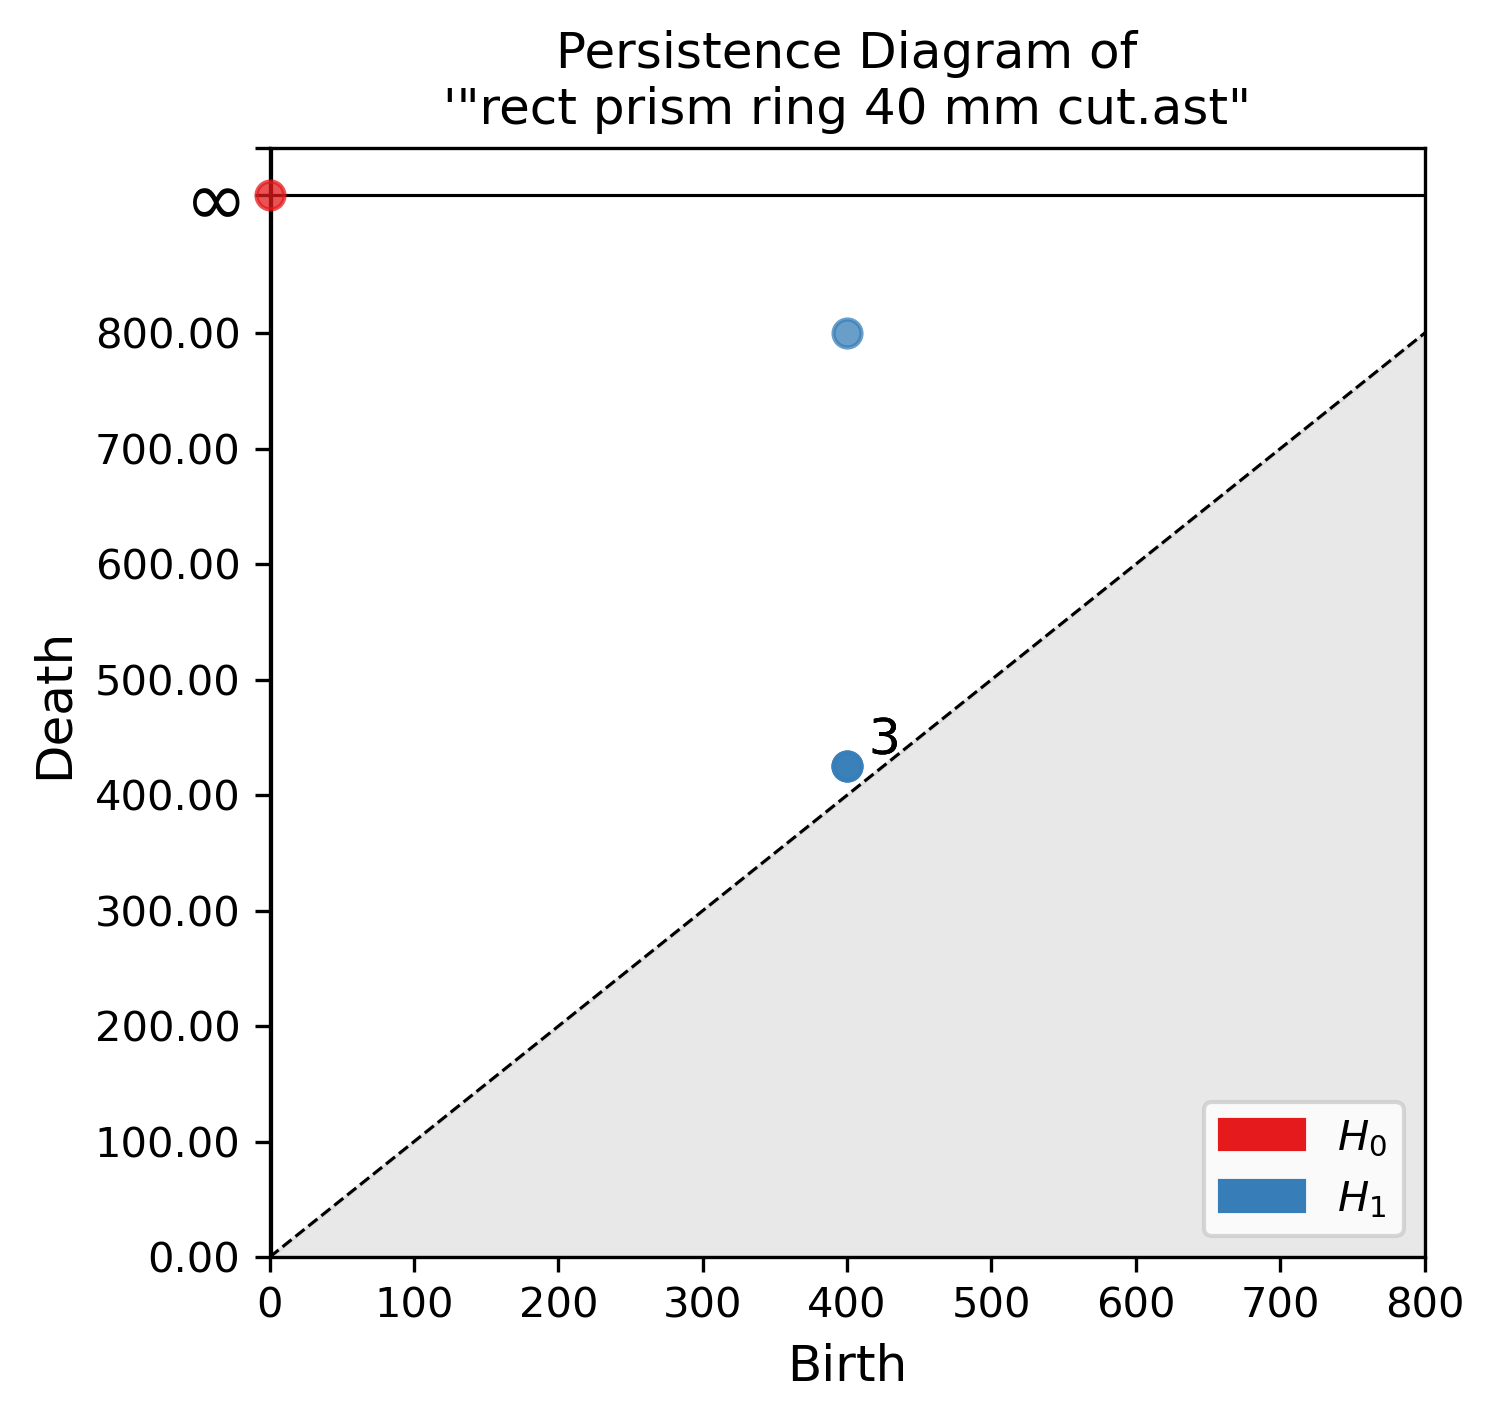
\includegraphics[width=1.875in]{Final Run, (rect prism ring 40 mm cut) persdia.png} &
         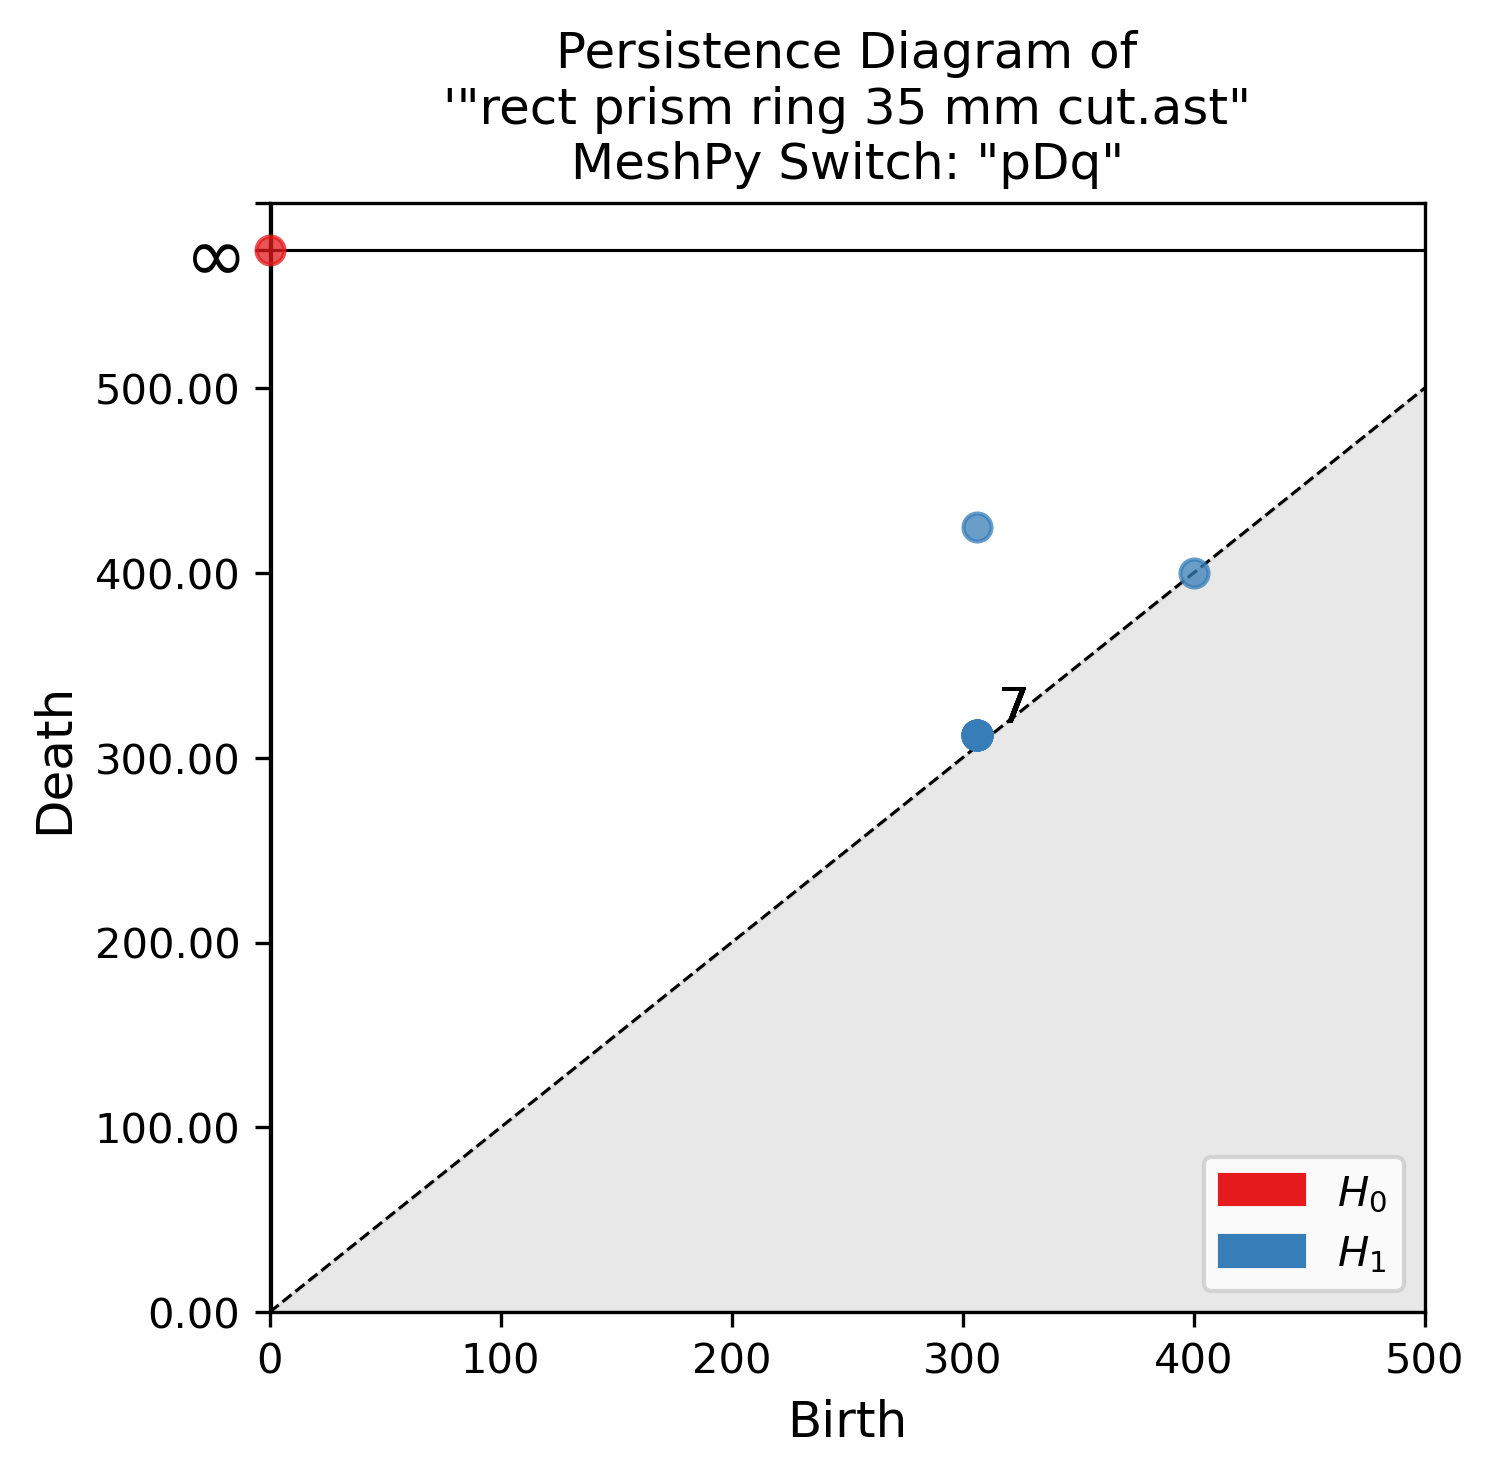
\includegraphics[width=1.875in]{Final Run, (rect prism ring 35 mm cut) persdia.png} &  
         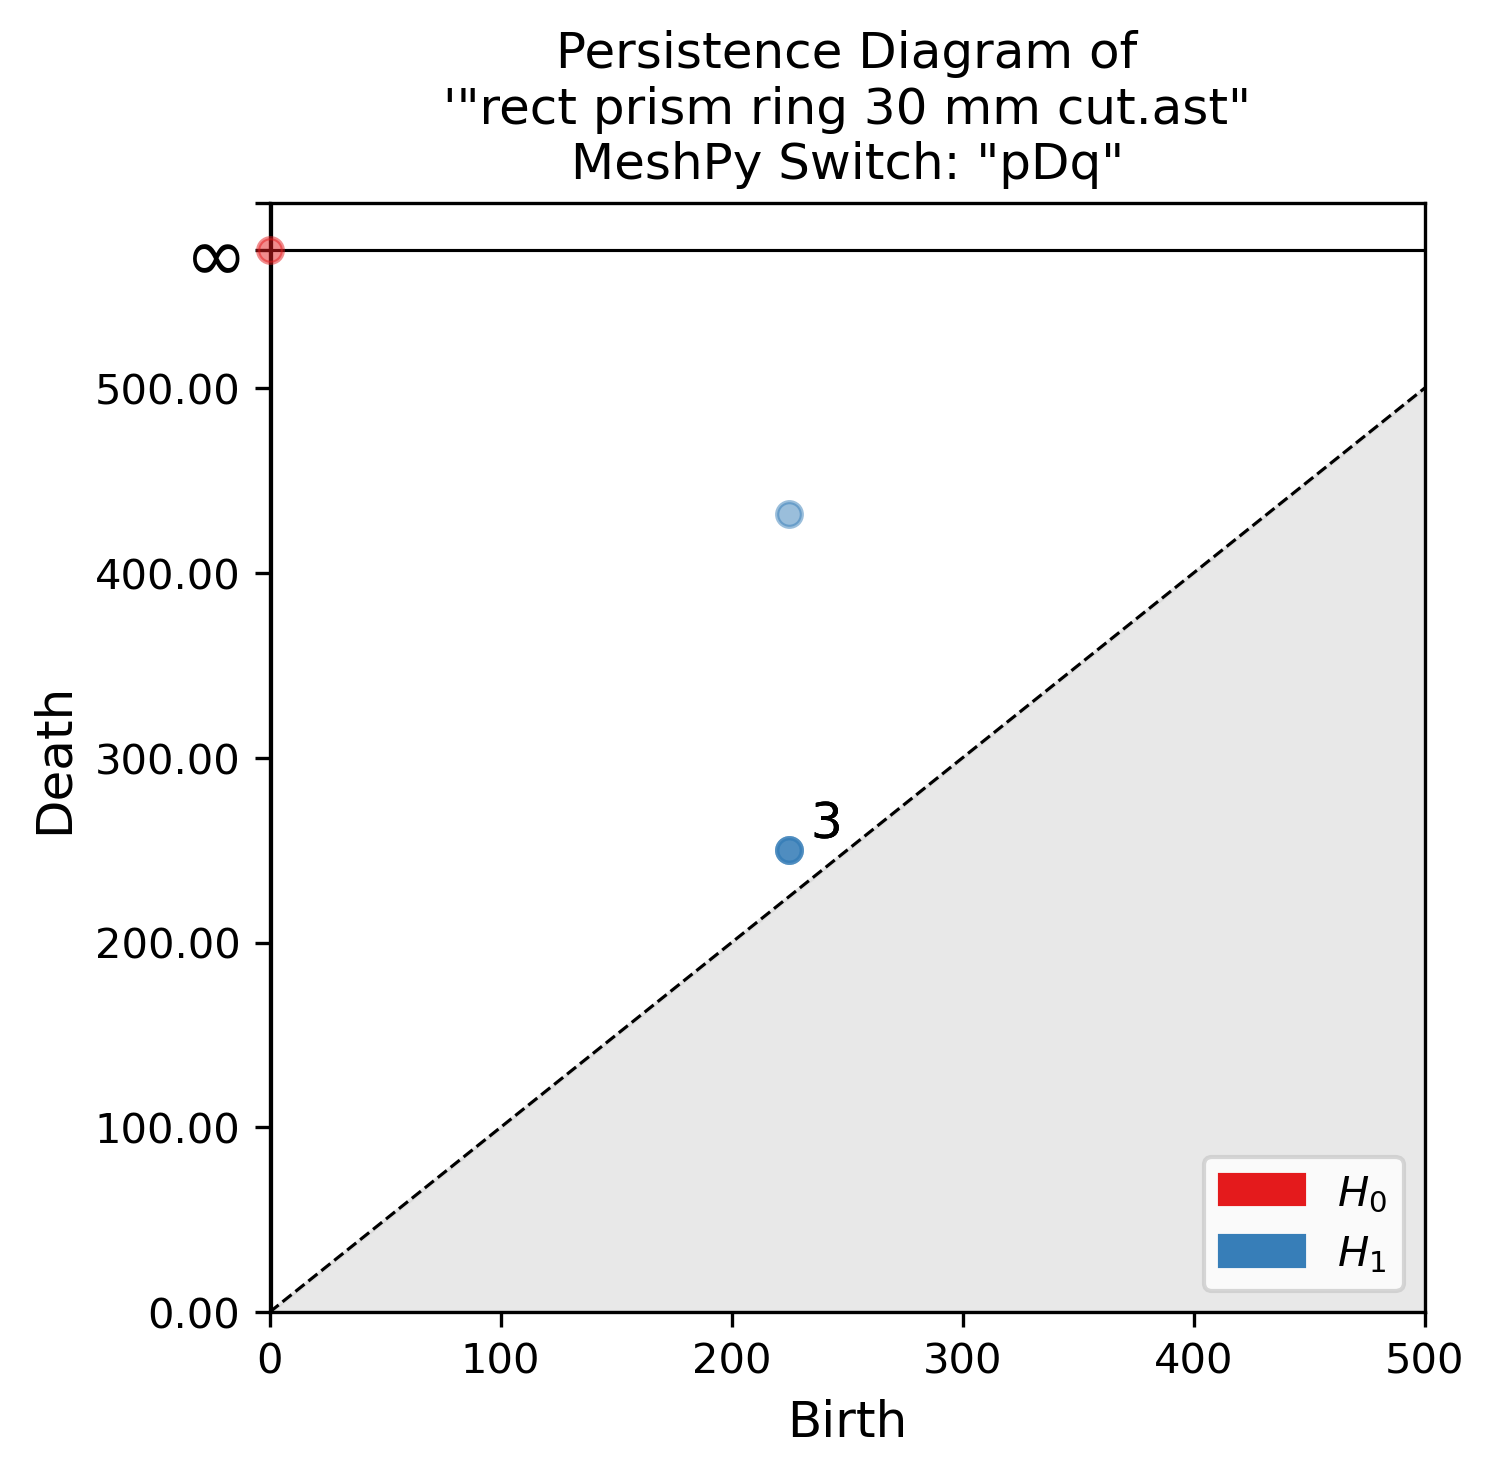
\includegraphics[width=1.875in]{Final Run, (rect prism ring 30 mm cut) persdia.png} \\
         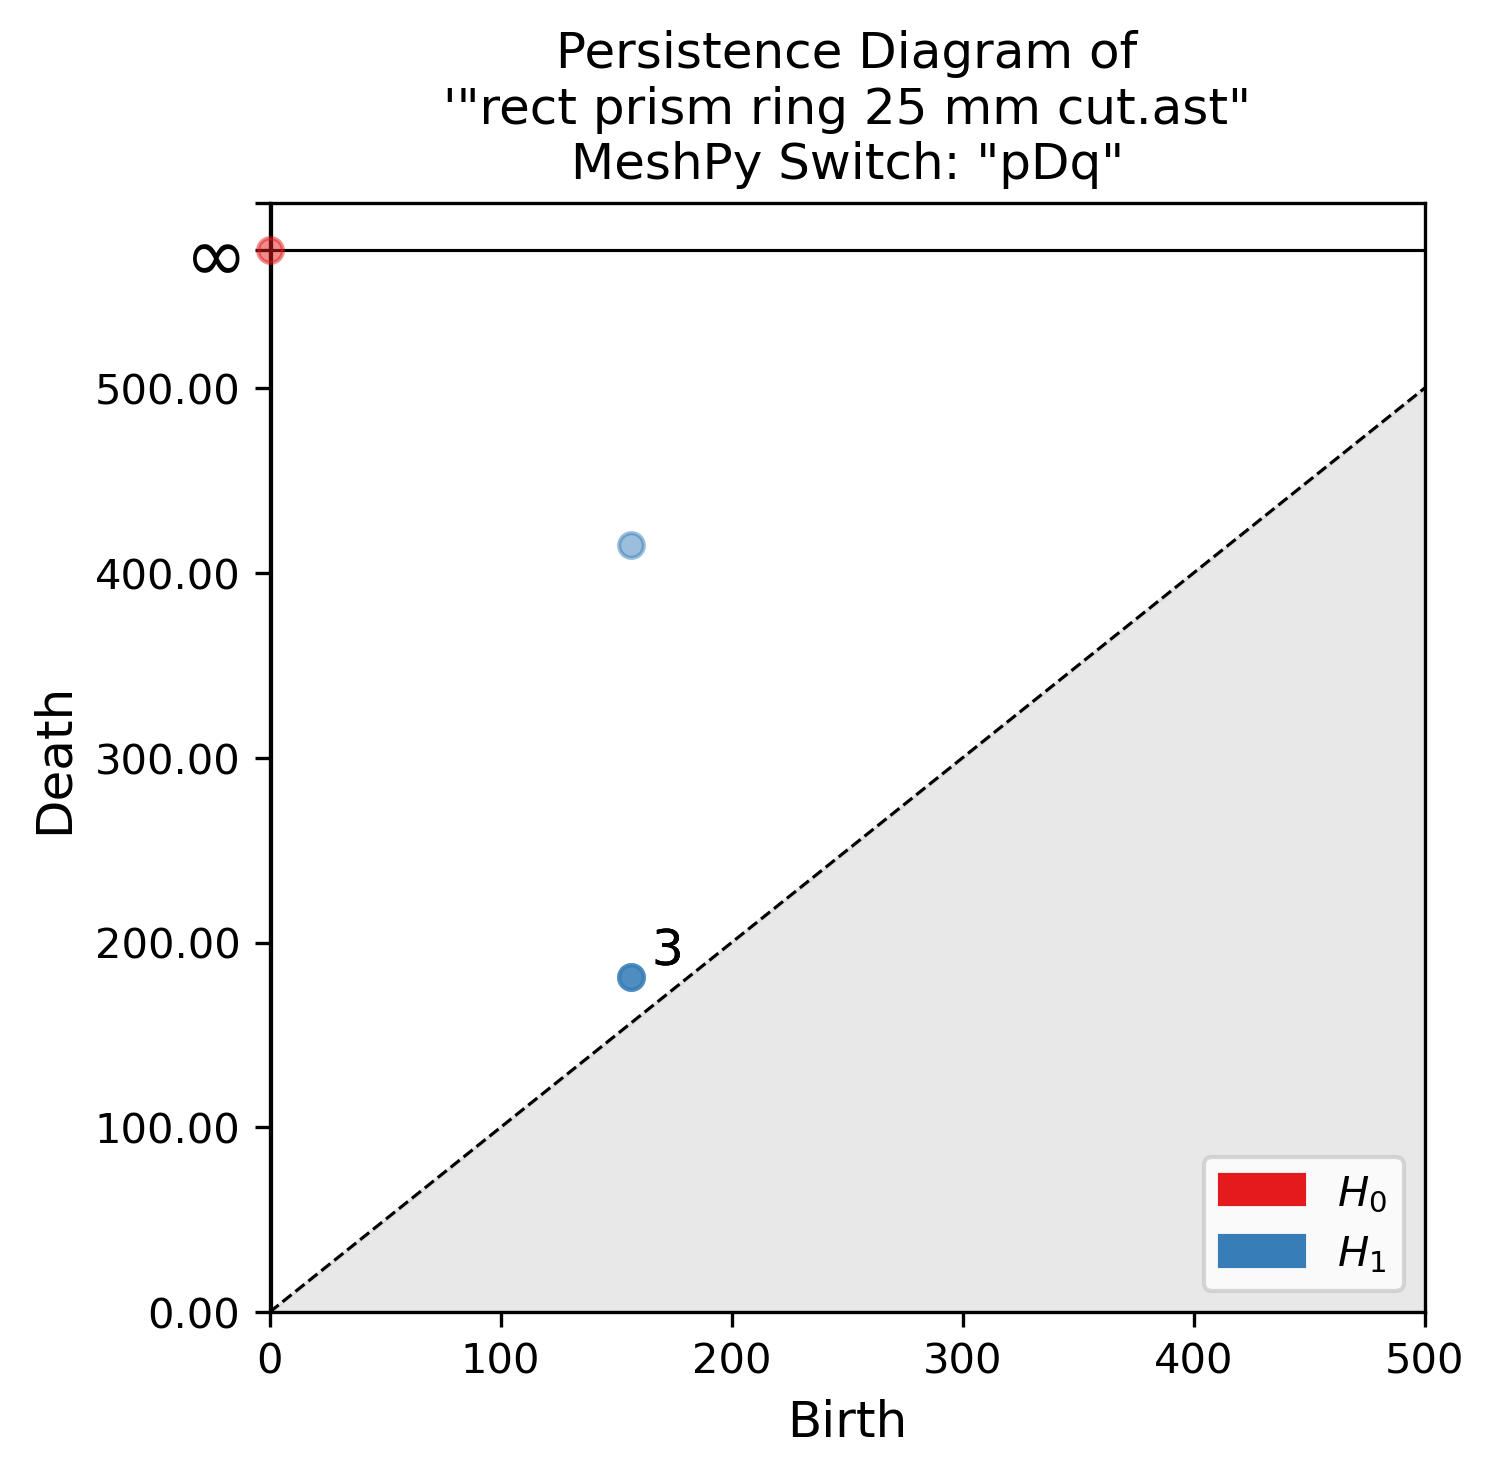
\includegraphics[width=1.875in]{Final Run, (rect prism ring 25 mm cut) persdia.png} & 
         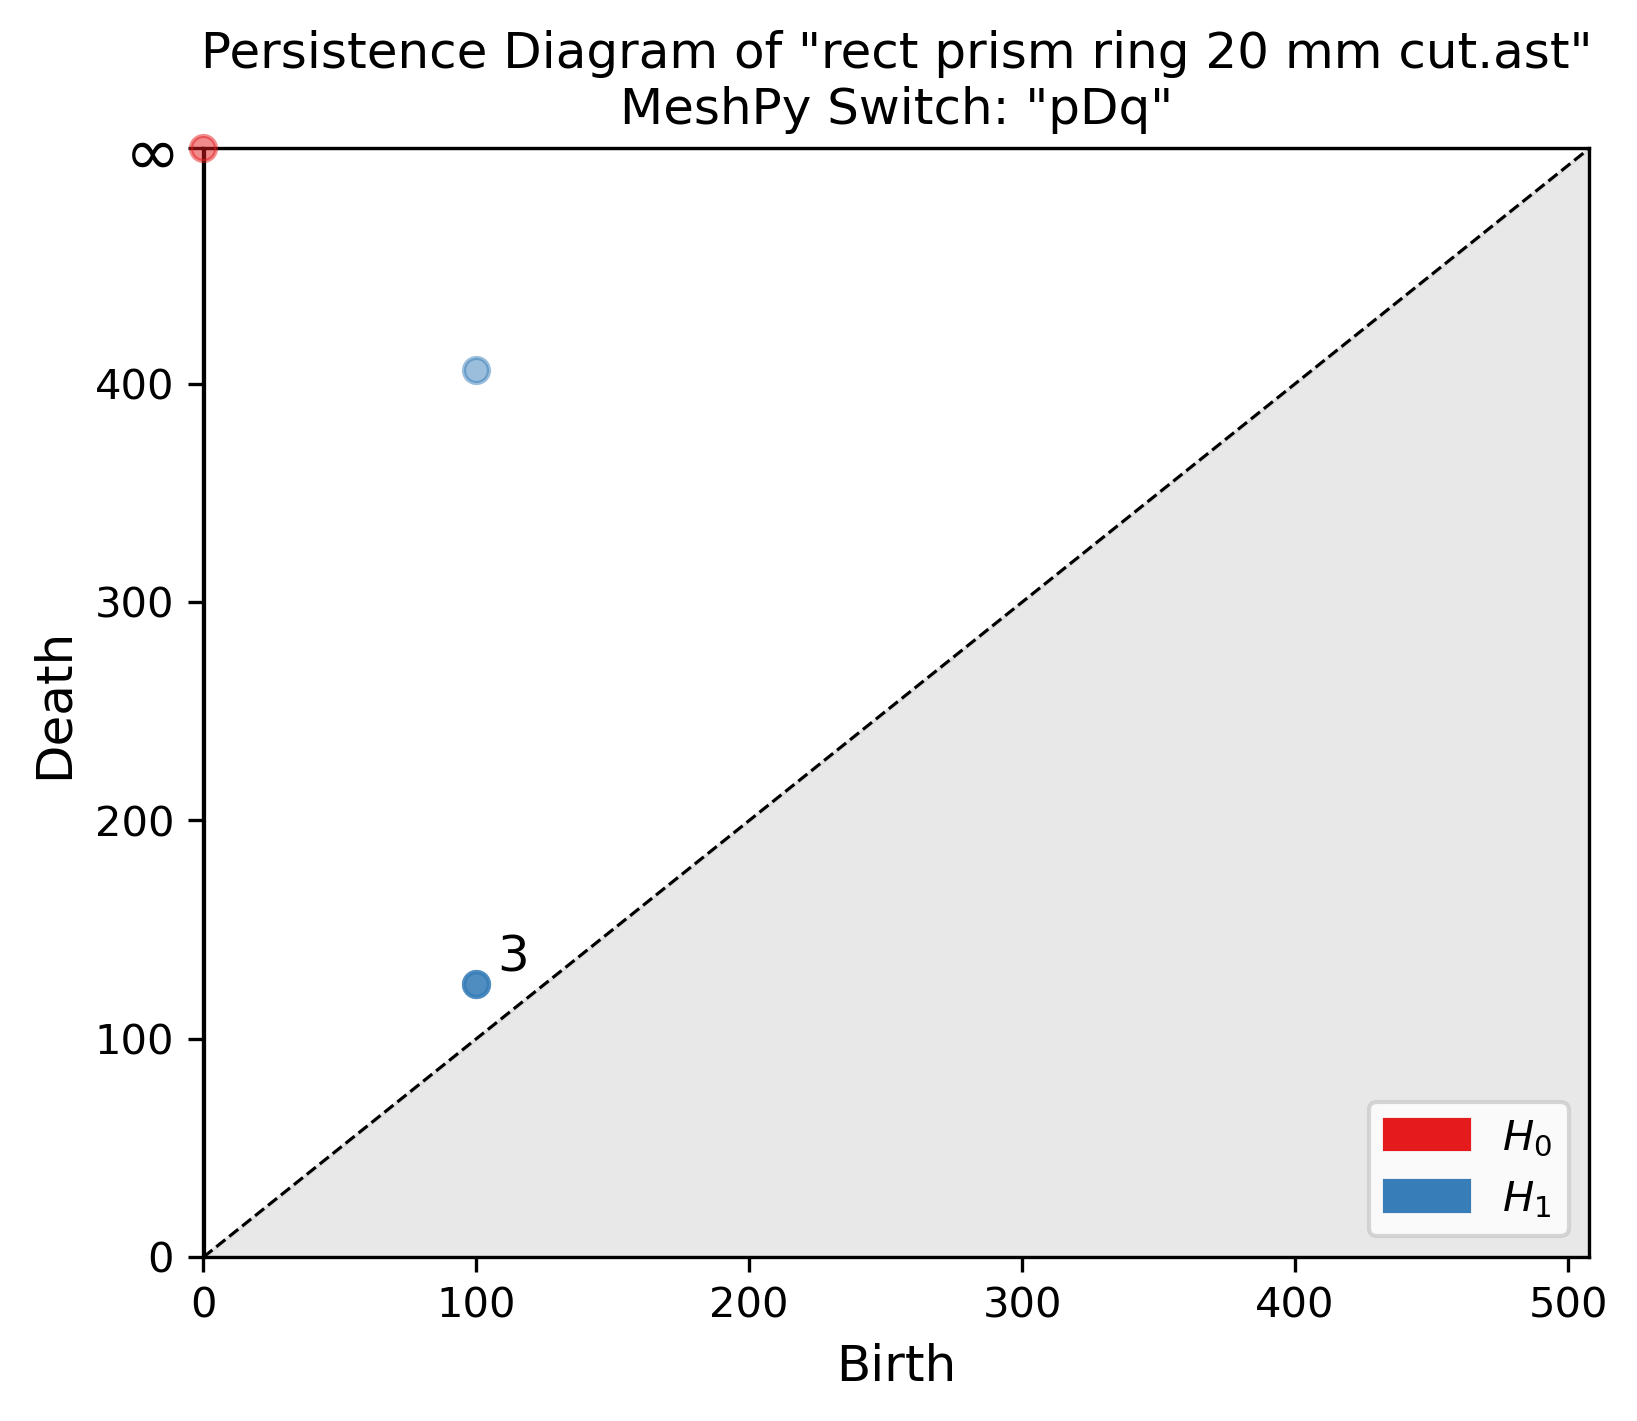
\includegraphics[width=1.875in]{Final Run, (rect prism ring 20 mm cut) persdia.png} & 
         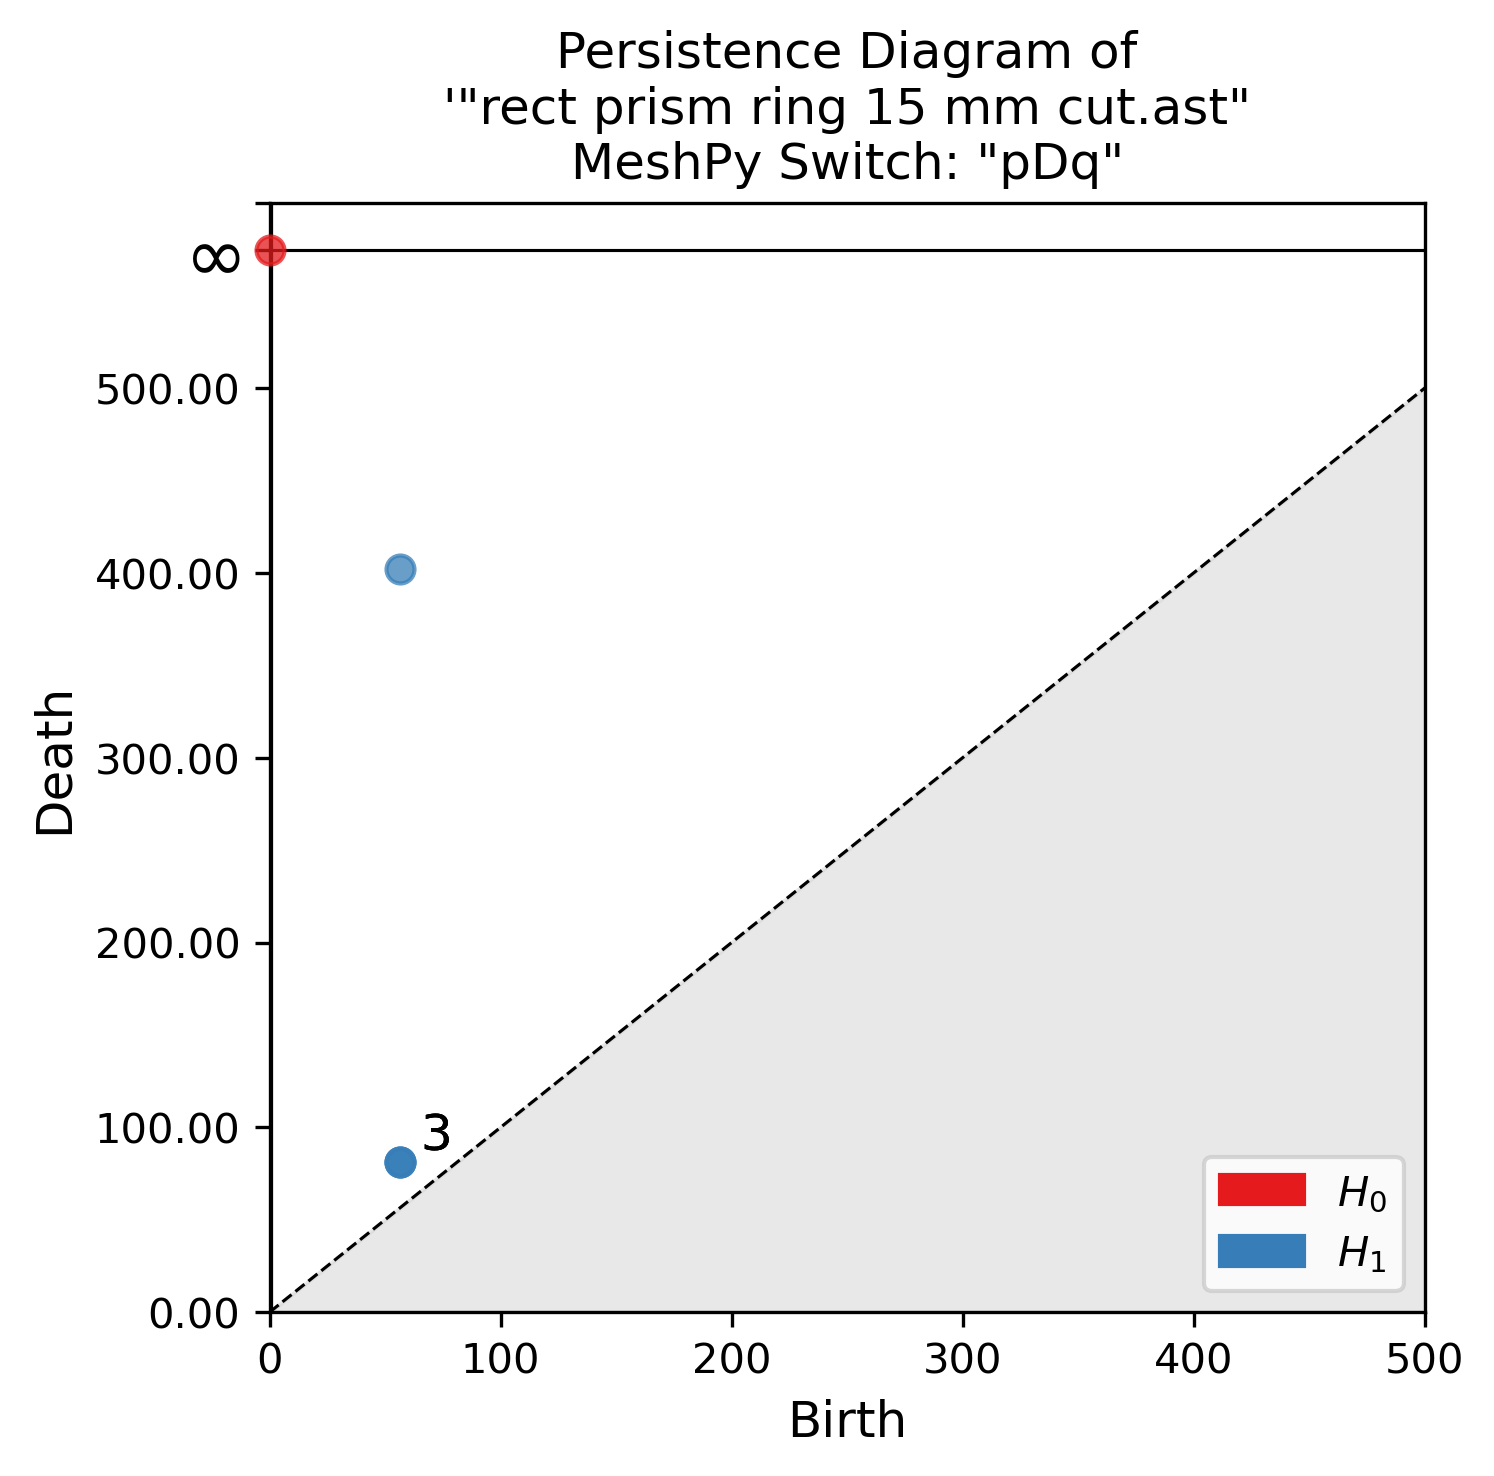
\includegraphics[width=1.875in]{Final Run, (rect prism ring 15 mm cut) persdia.png} \\
         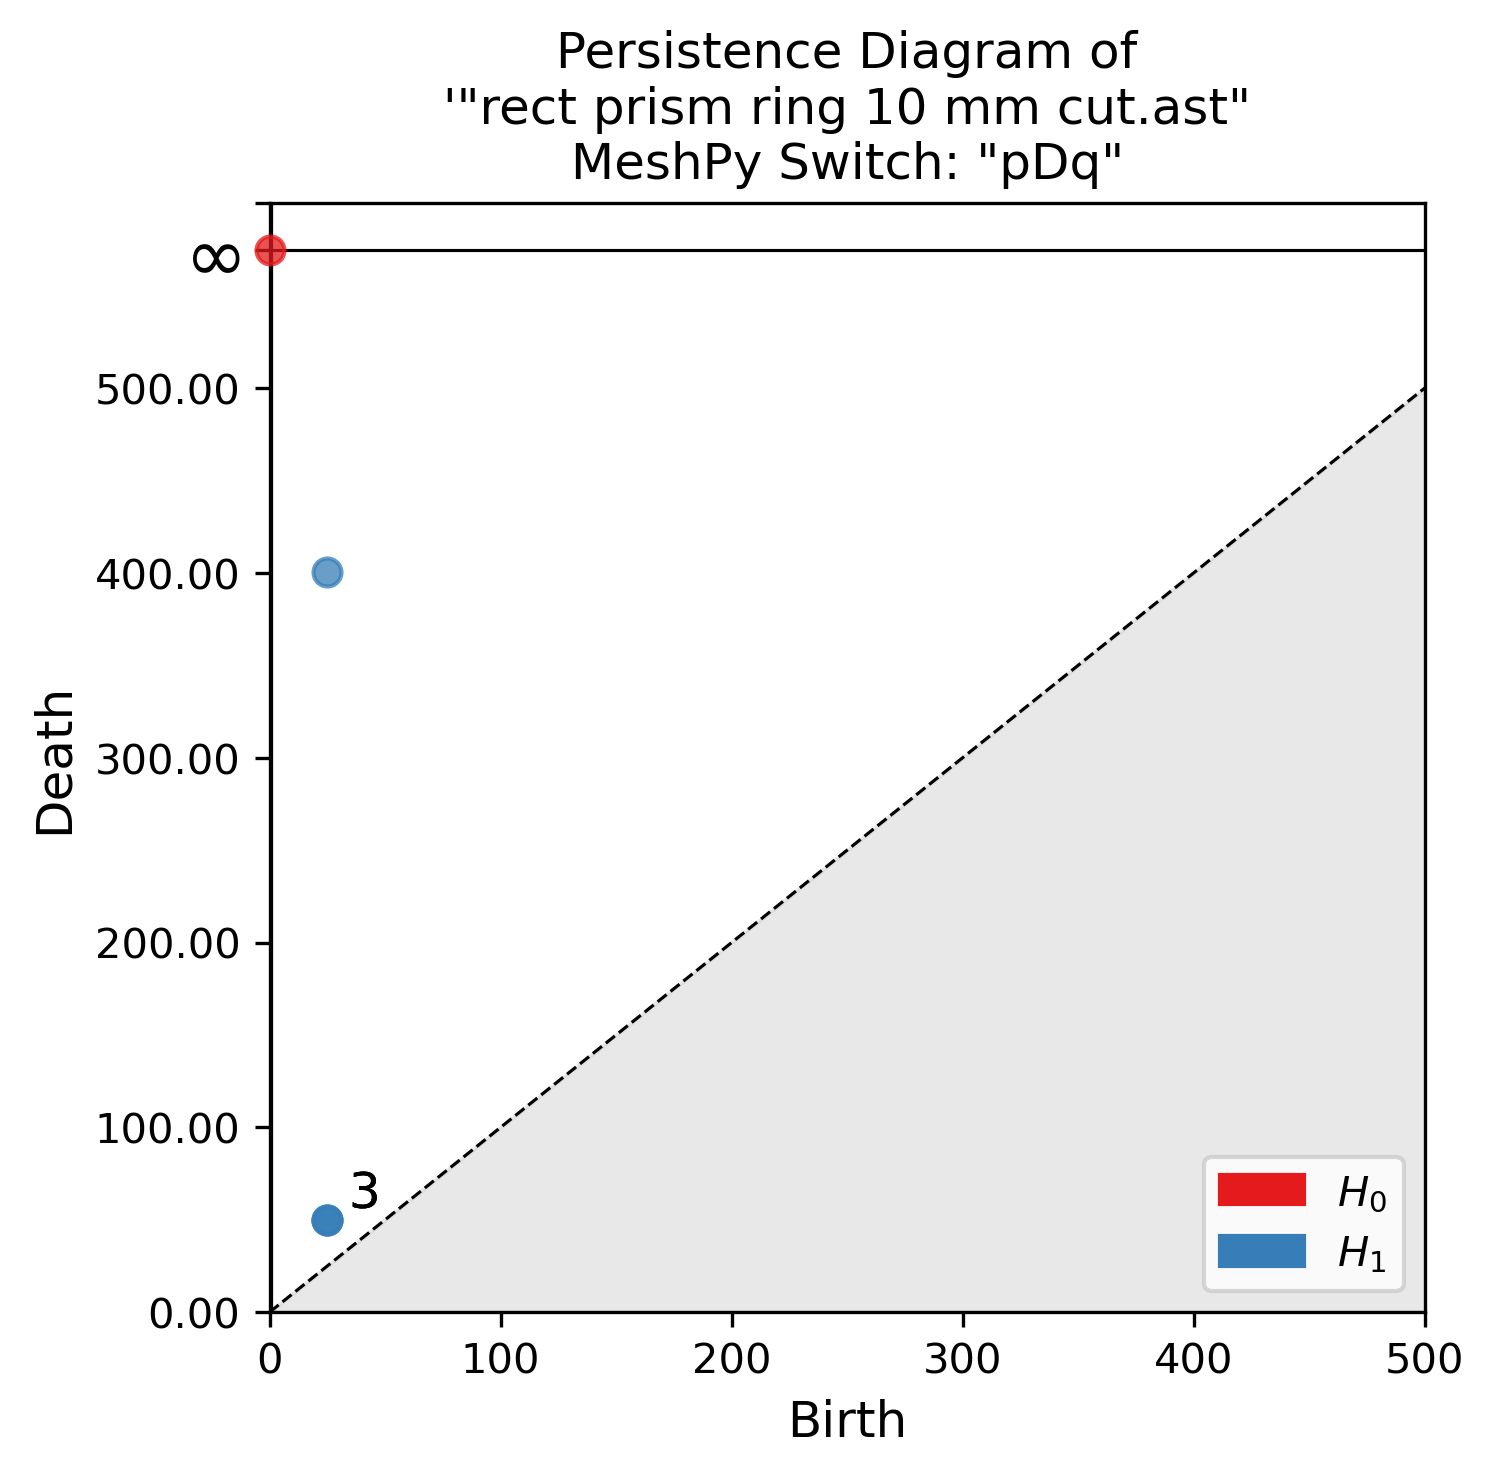
\includegraphics[width=1.875in]{Final Run, (rect prism ring 10 mm cut) persdia.png} & 
         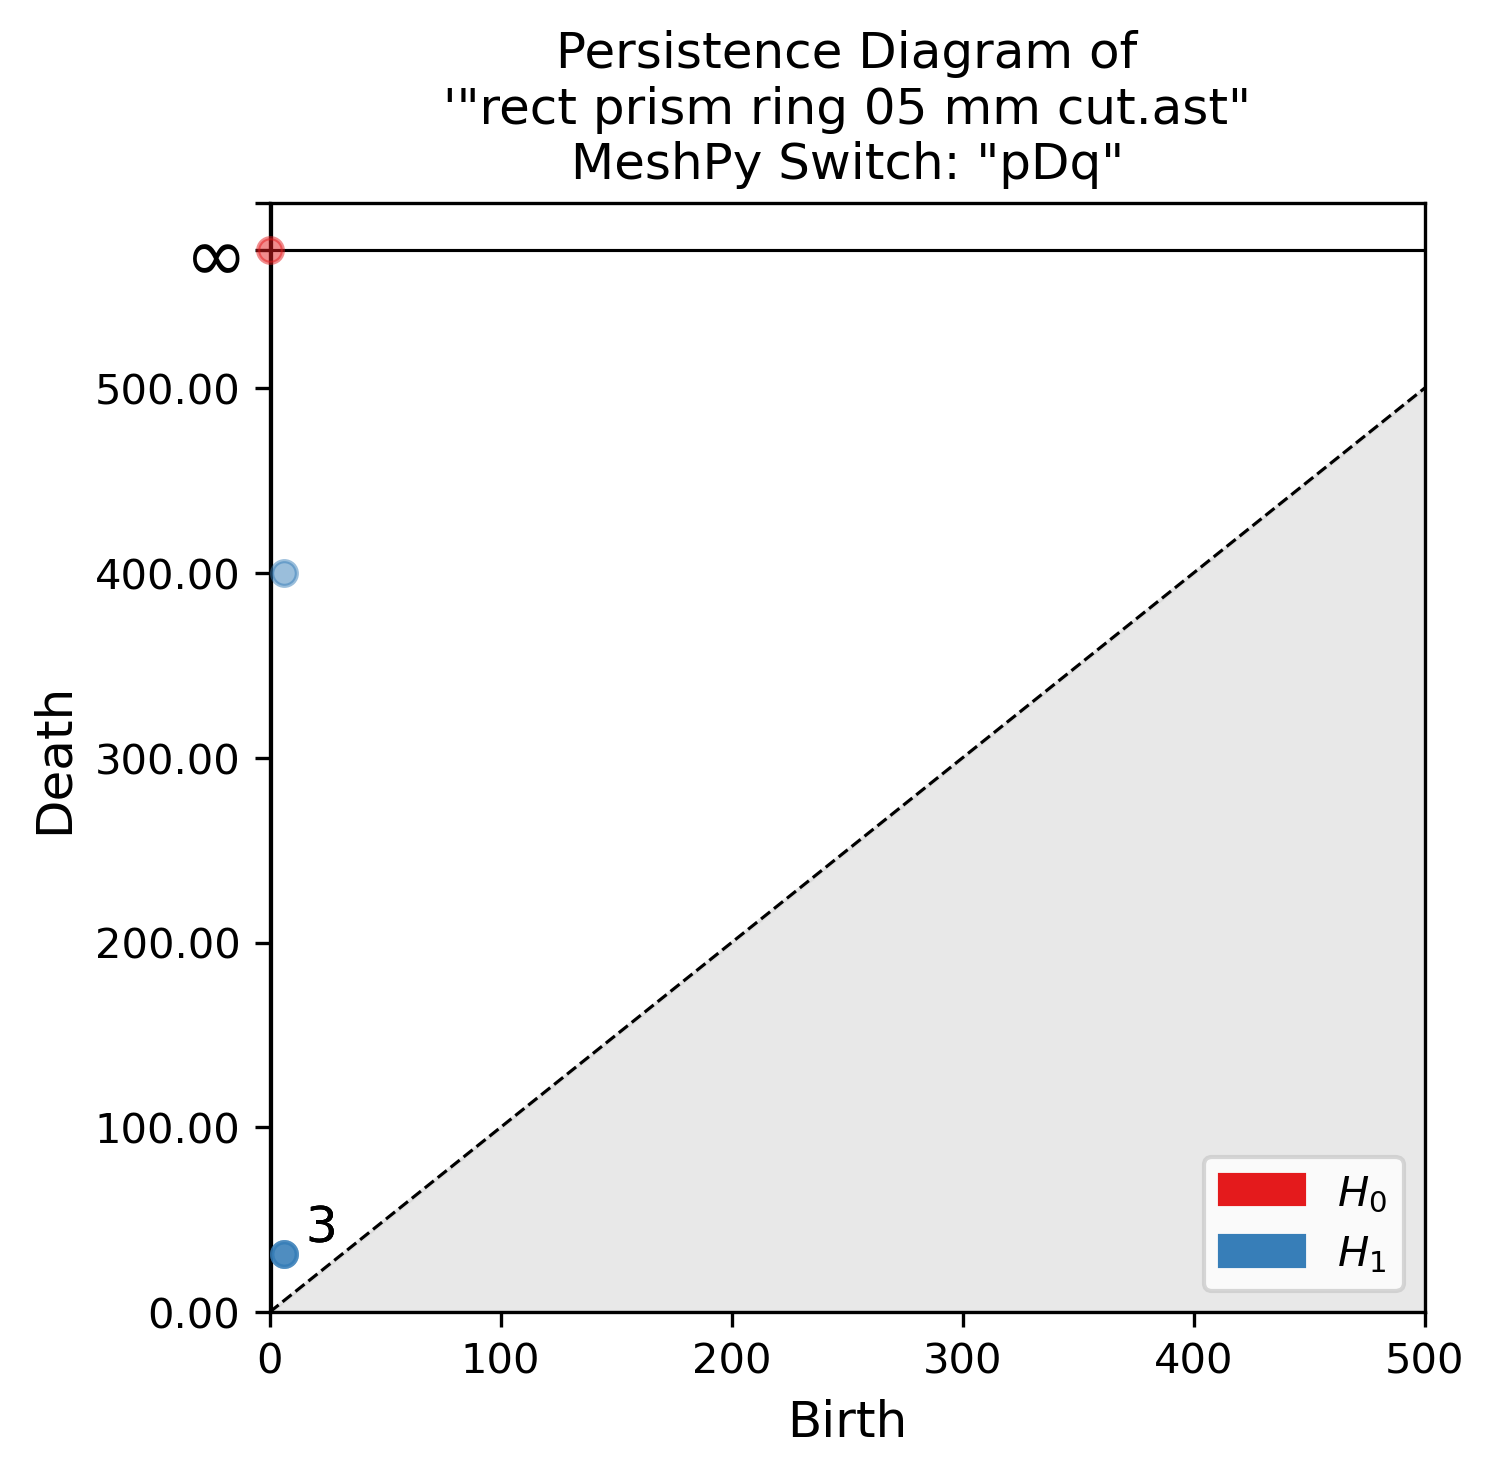
\includegraphics[width=1.875in]{Final Run, (rect prism ring 05 mm cut) persdia.png} & 
         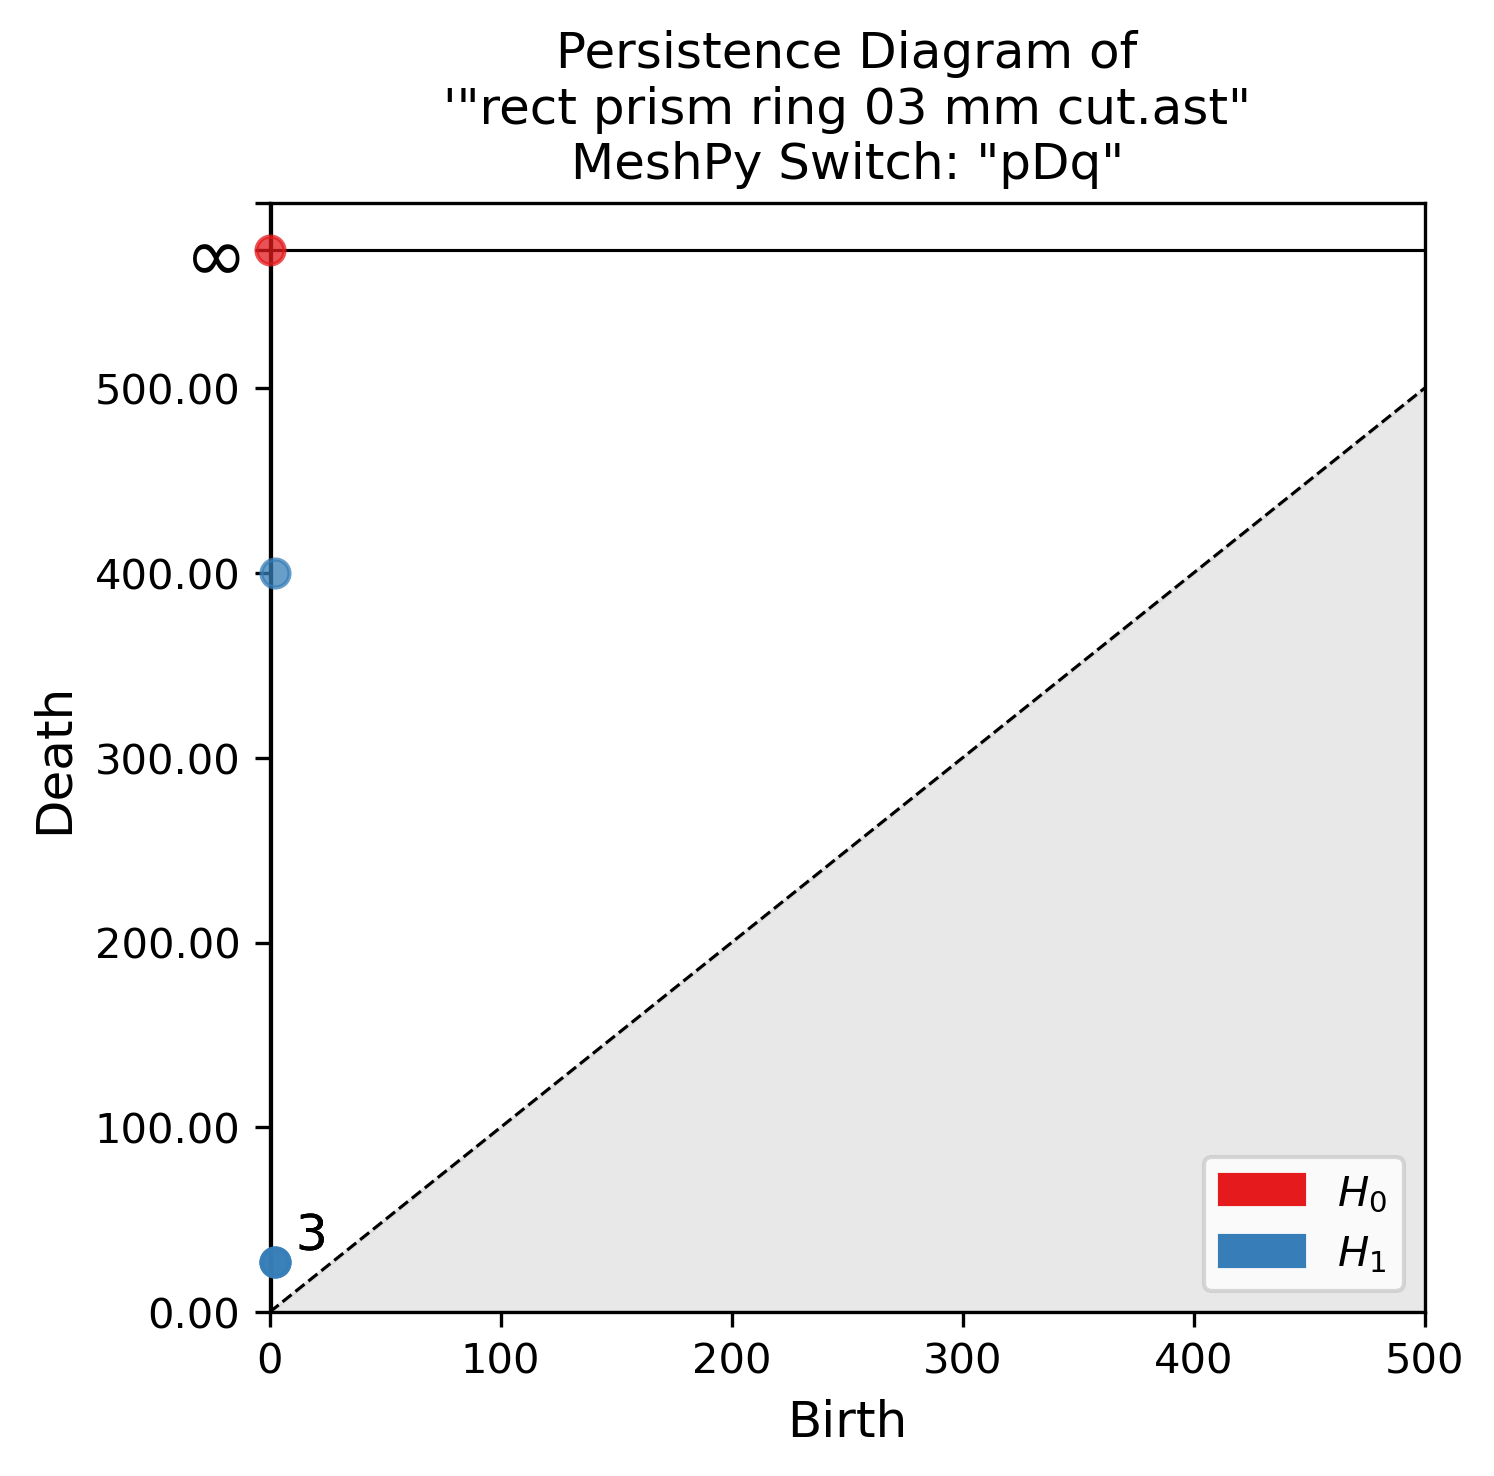
\includegraphics[width=1.875in]{Final Run, (rect prism ring 03 mm cut) persdia.png} \\
         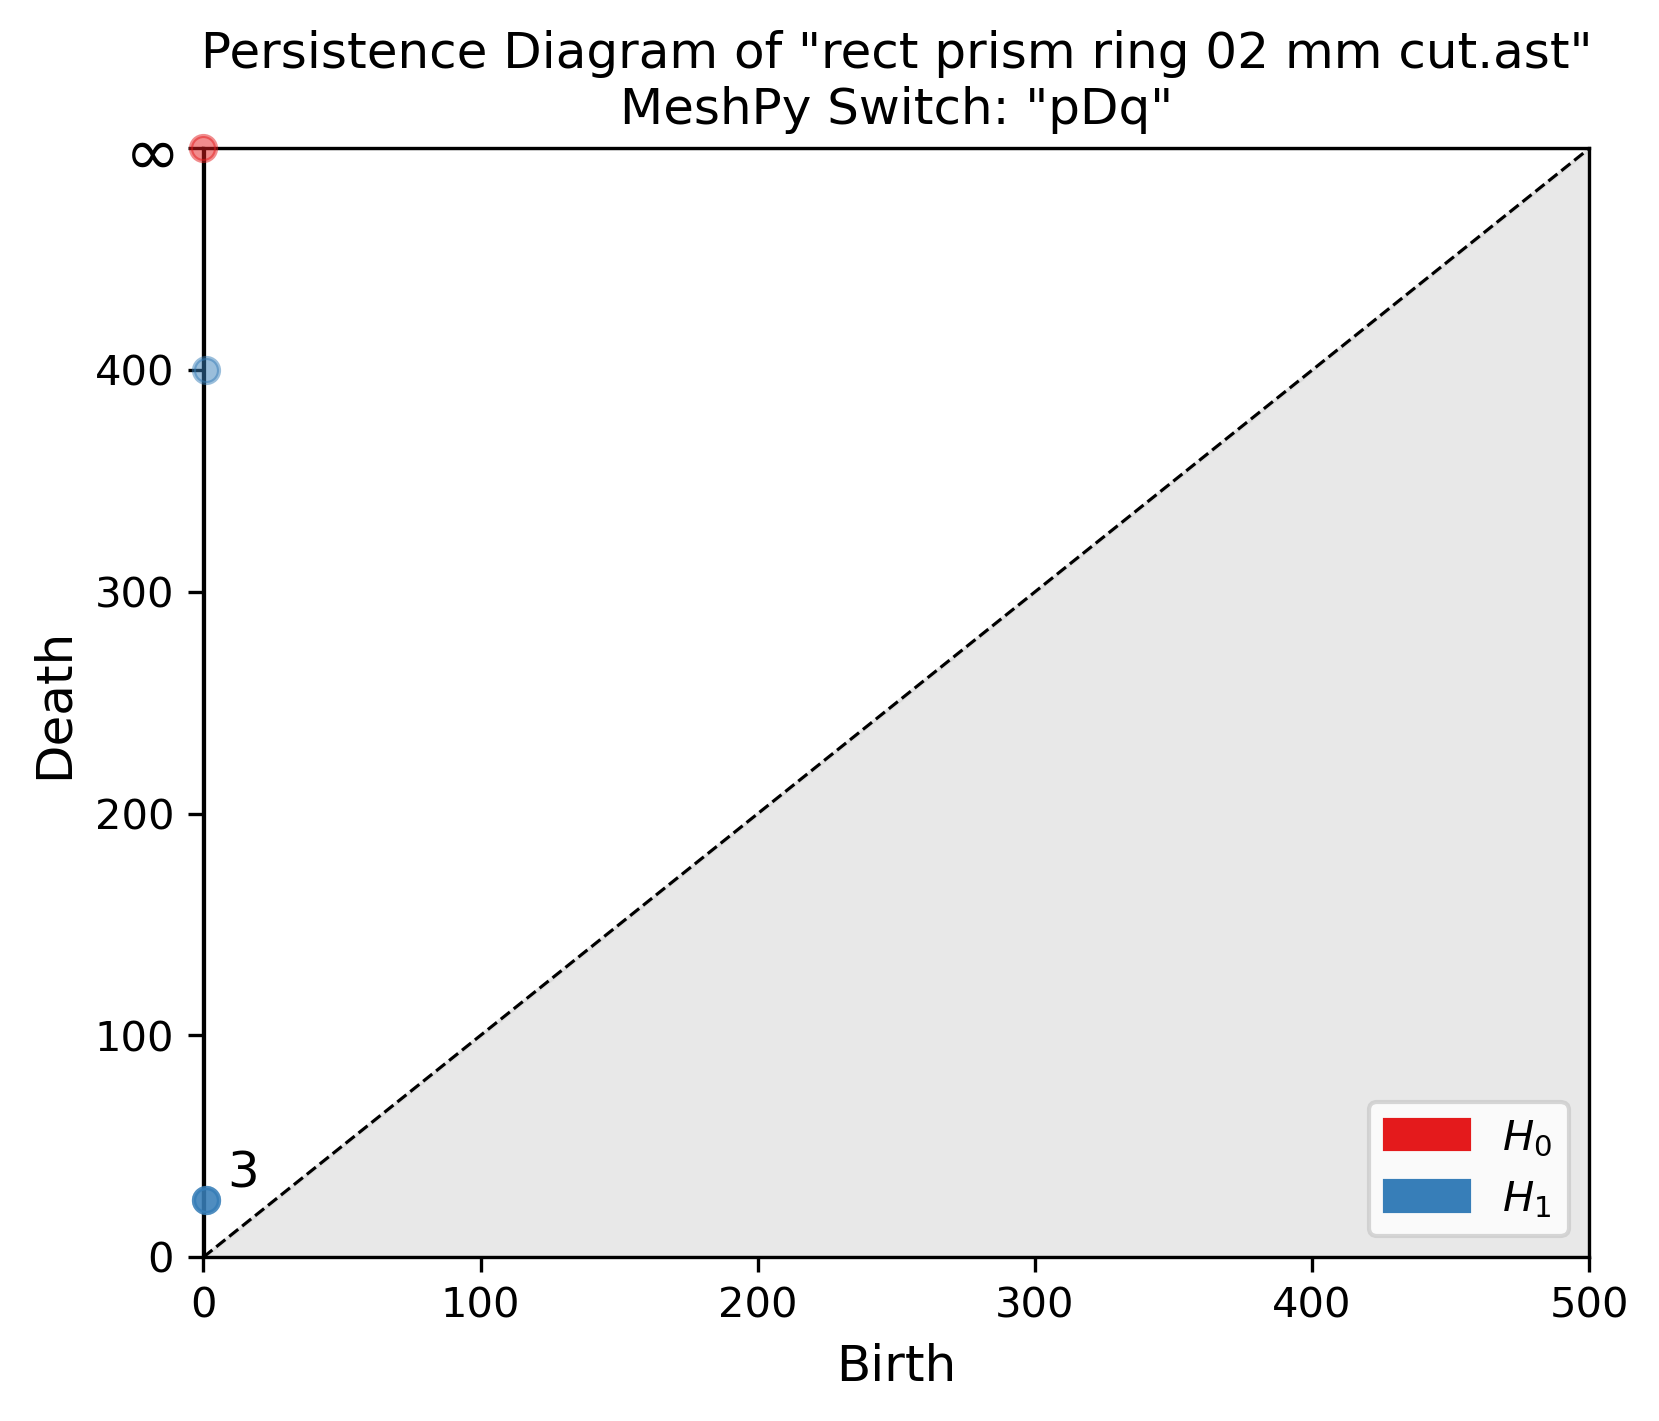
\includegraphics[width=1.875in]{Final Run, (rect prism ring 02 mm cut) persdia.png} &
         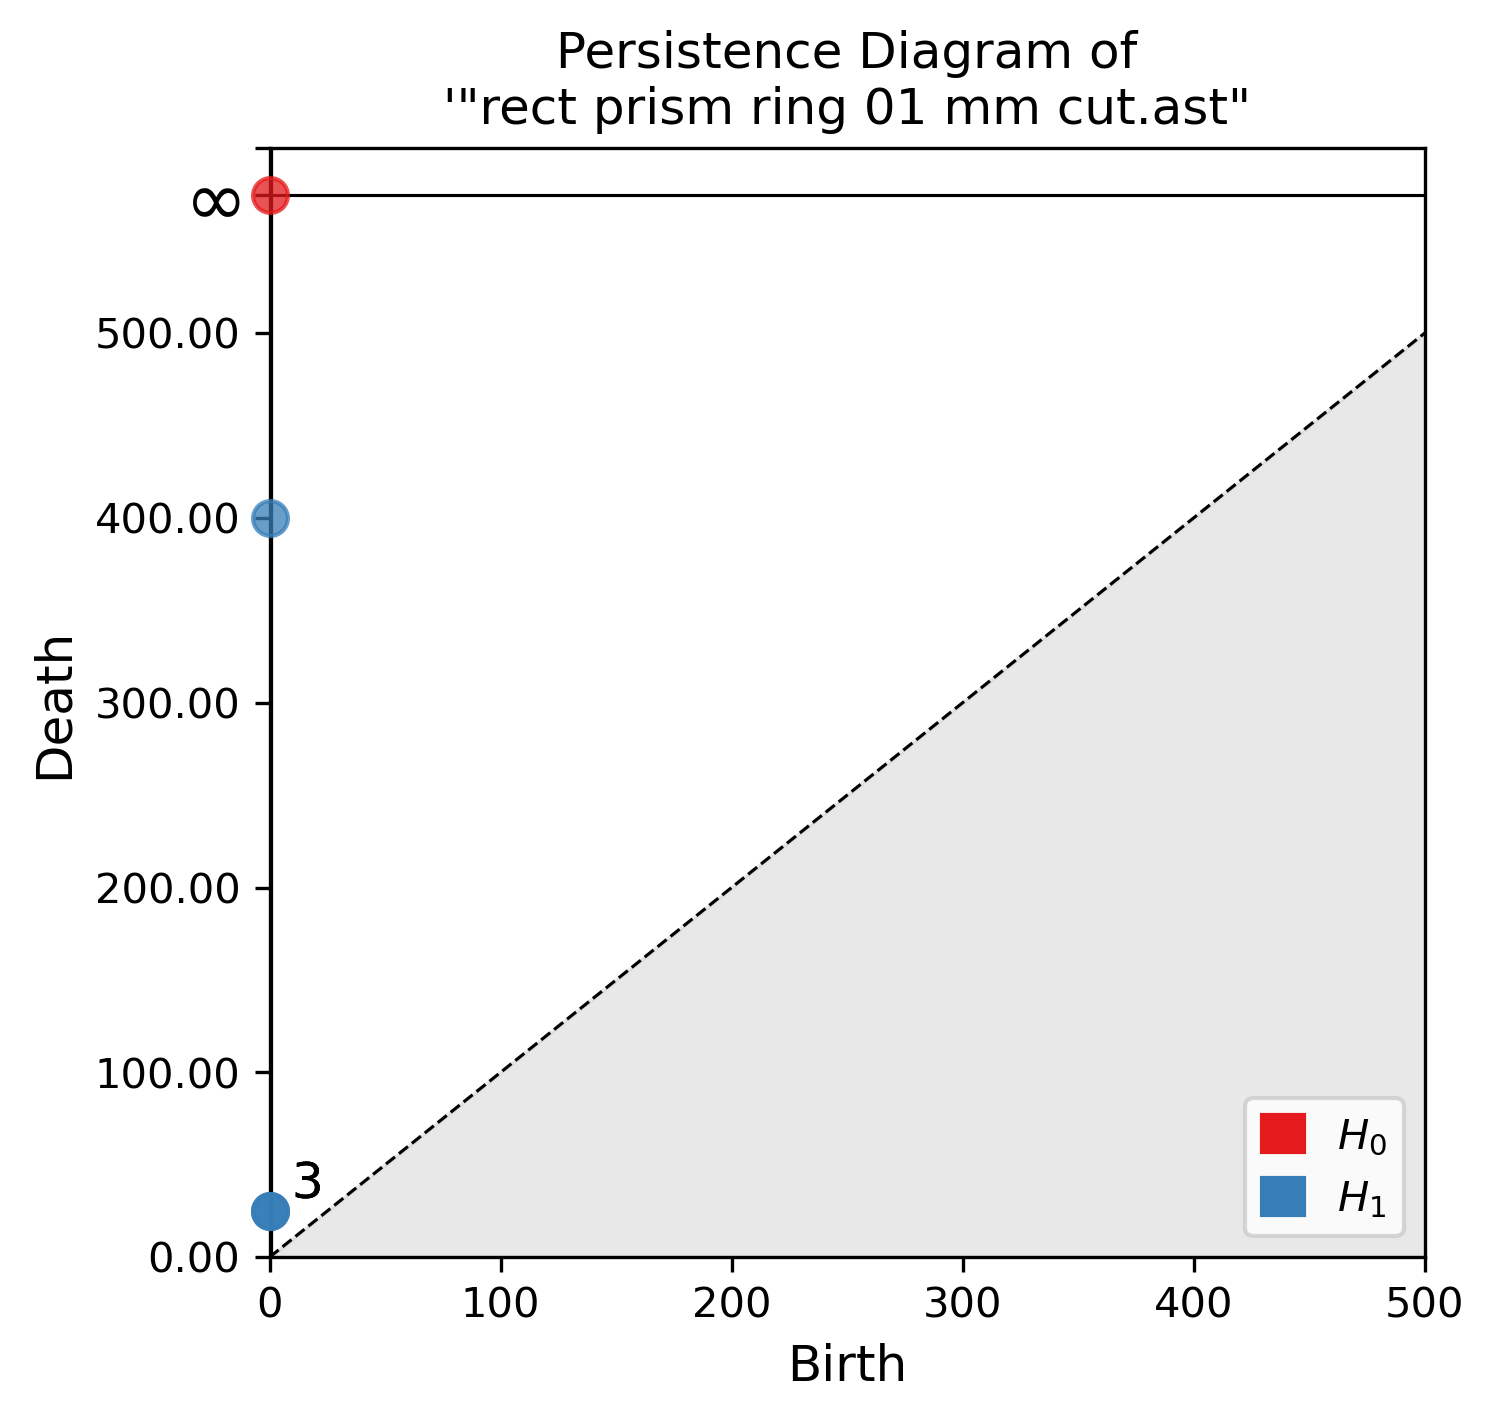
\includegraphics[width=1.875in]{Final Run, (rect prism ring 01 mm cut) persdia.png} &
         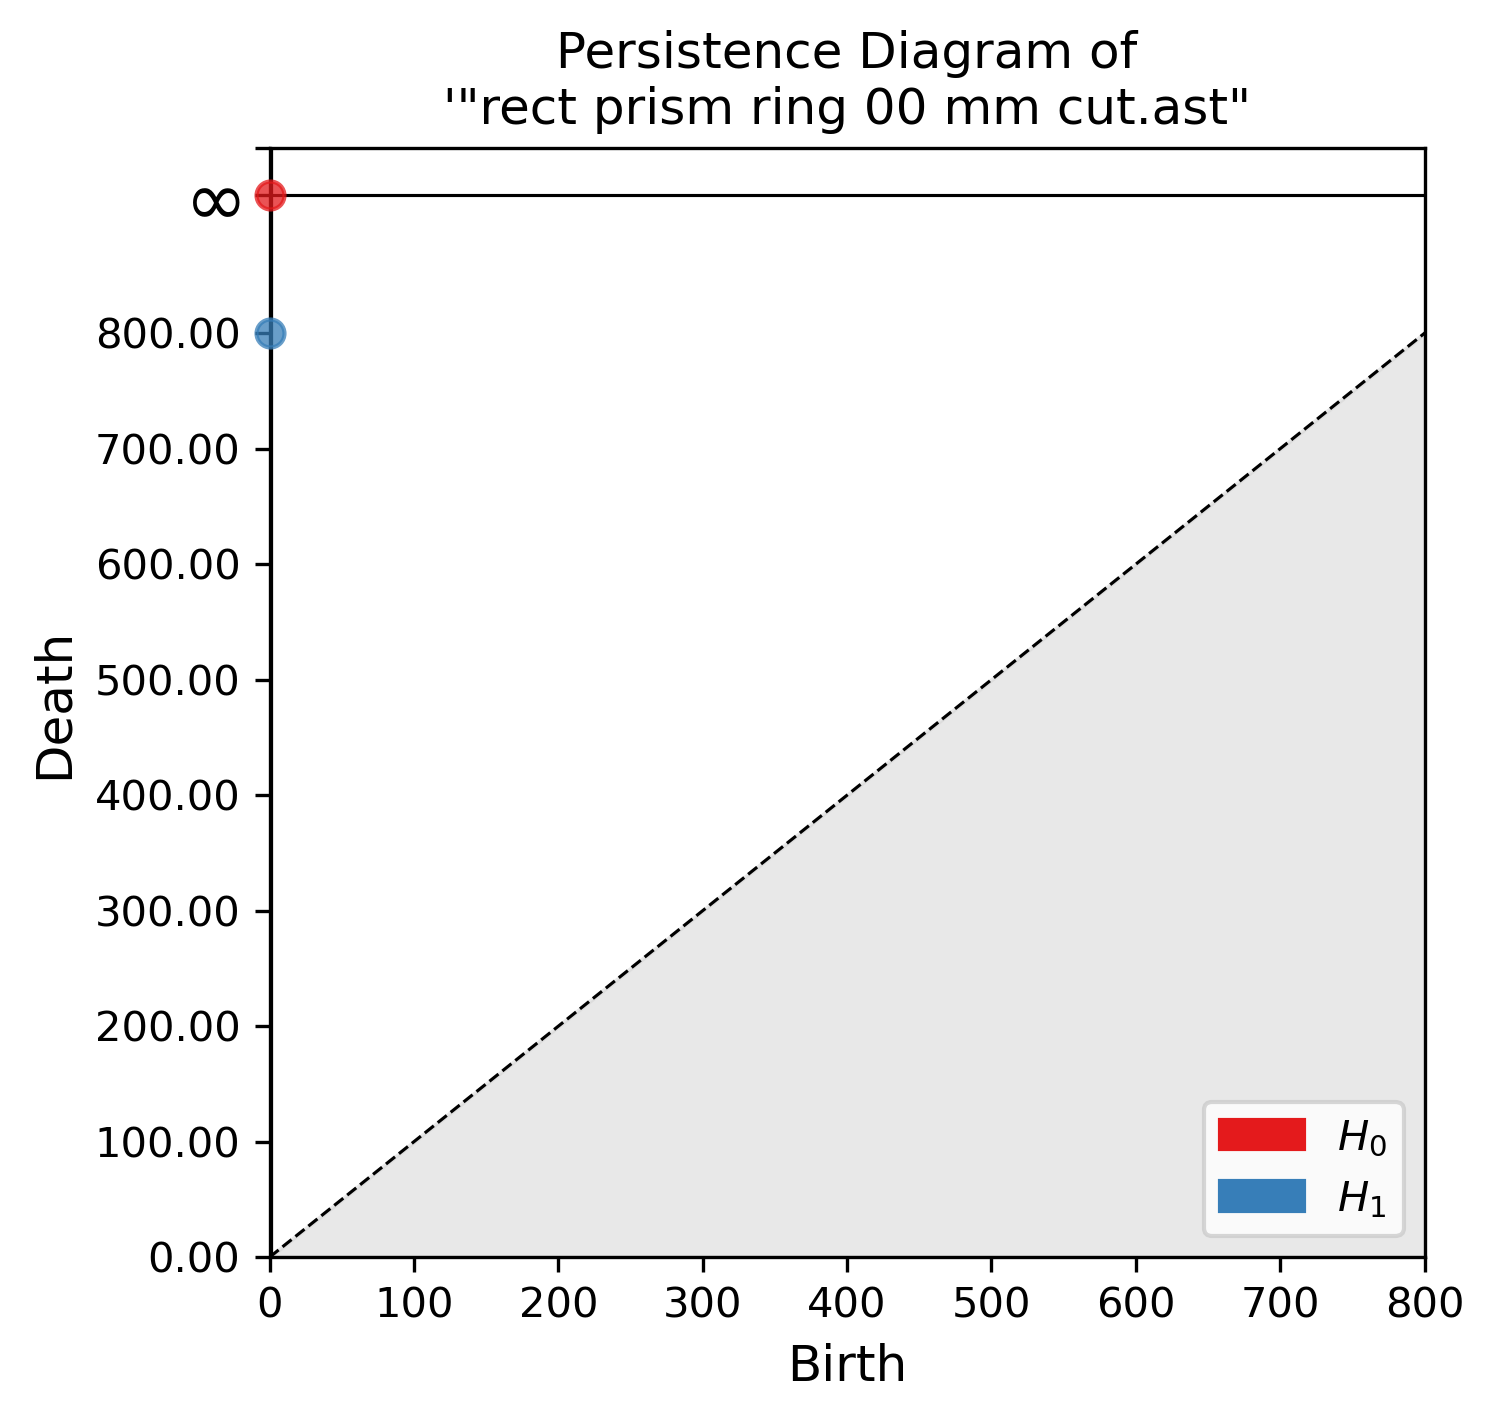
\includegraphics[width=1.875in]{Final Run, (rect prism ring 00 mm cut) persdia.png} \\
    \end{tabular}
    \end{center}
    \caption{Persistence Diagrams of a rectangular prism ring with a cut that decreases to the original shape.}
    \label{fig:rect_prism_ring_persdia_table}
\end{table}

\newpage
\section{Two Cubes with Three Pockets Moving Closer}
A pocket operation in CAD can create a hole which goes through an object. This operation was done to a cube on the top, front, and right faces to create three intersecting pockets, as shown below.
\begin{figure}[H]
\begin{center}
	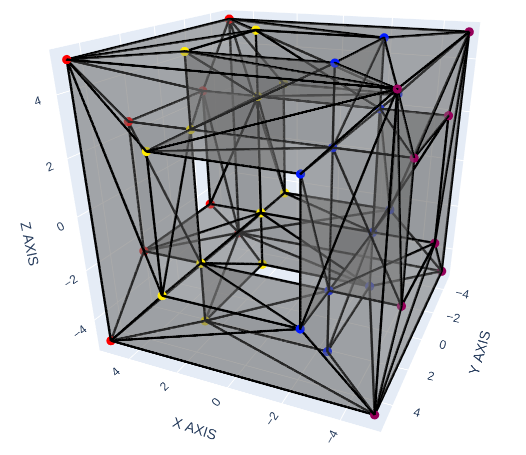
\includegraphics[height=1.25in]{one cube three pockets each.png}
    \caption{3D plot of an ASCII STL file of an individual cube with three pockets.}
\label{fig:ast_tetrahedrons}
\end{center}
\end{figure}

\begin{table}[H]
    \begin{center}
    \begin{tabular}{|c|c|}
    \toprule
    \tstack{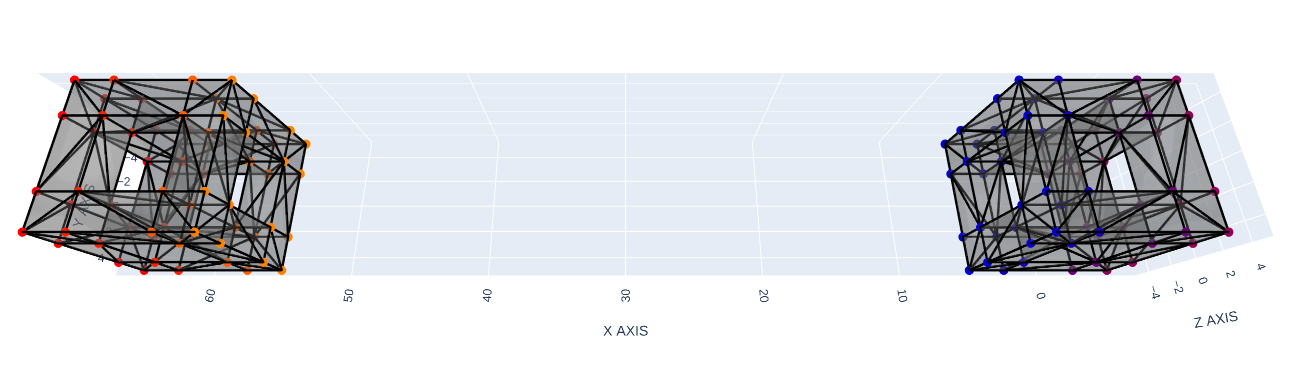
\includegraphics[width=3in]{Final Run, (two cubes, three pockets each, 50 mm apart) meshpy plotly screenshots.png}\\ {\fontsize{10}{12}\selectfont 50 mm apart}}  &
    \tstack{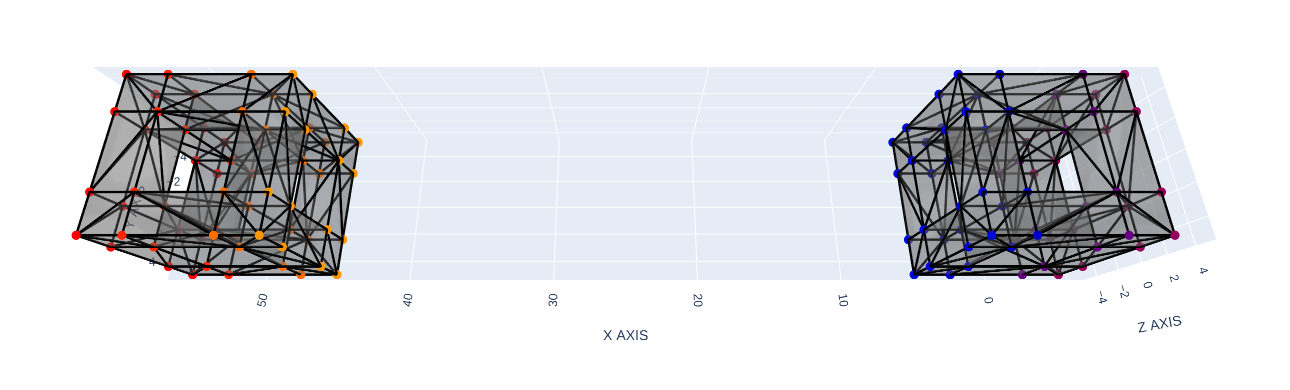
\includegraphics[width=3in]{Final Run, (two cubes, three pockets each, 40 mm apart) meshpy plotly screenshots.png}\\ {\fontsize{10}{12}\selectfont 40 mm apart}}  \\
    \midrule
	\tstack{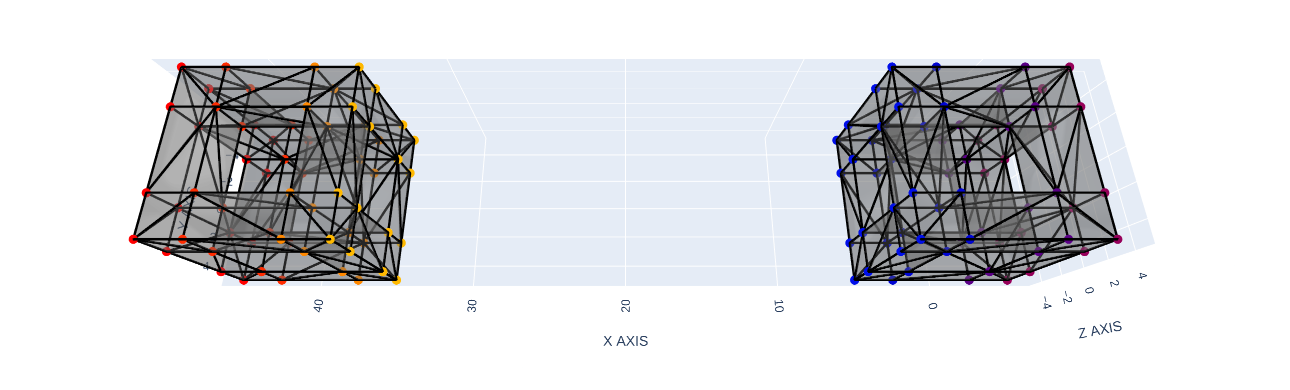
\includegraphics[width=3in]{Final Run, (two cubes, three pockets each, 30 mm apart) meshpy plotly screenshots.png}\\ {\fontsize{10}{12}\selectfont 30 mm apart}}   &
	\tstack{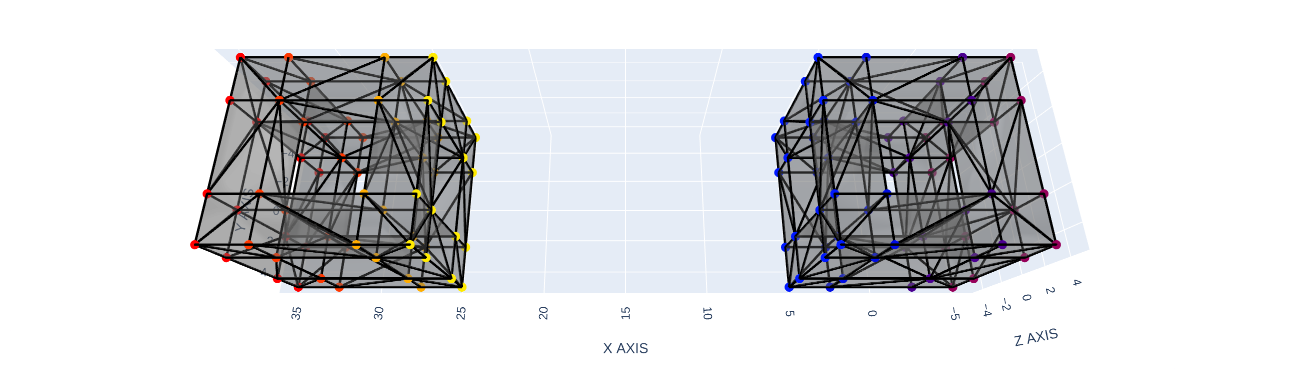
\includegraphics[width=3in]{Final Run, (two cubes, three pockets each, 20 mm apart) meshpy plotly screenshots.png}\\ {\fontsize{10}{12}\selectfont 20 mm apart}}  \\
	\midrule
    \tstack{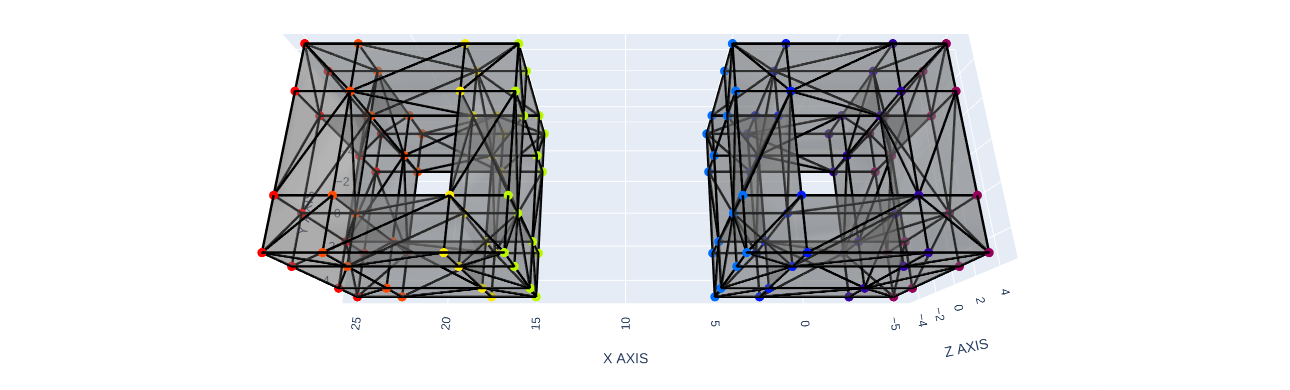
\includegraphics[width=3in]{Final Run, (two cubes, three pockets each, 10 mm apart) meshpy plotly screenshots.png}\\ {\fontsize{10}{12}\selectfont 10 mm apart}}  &
    \tstack{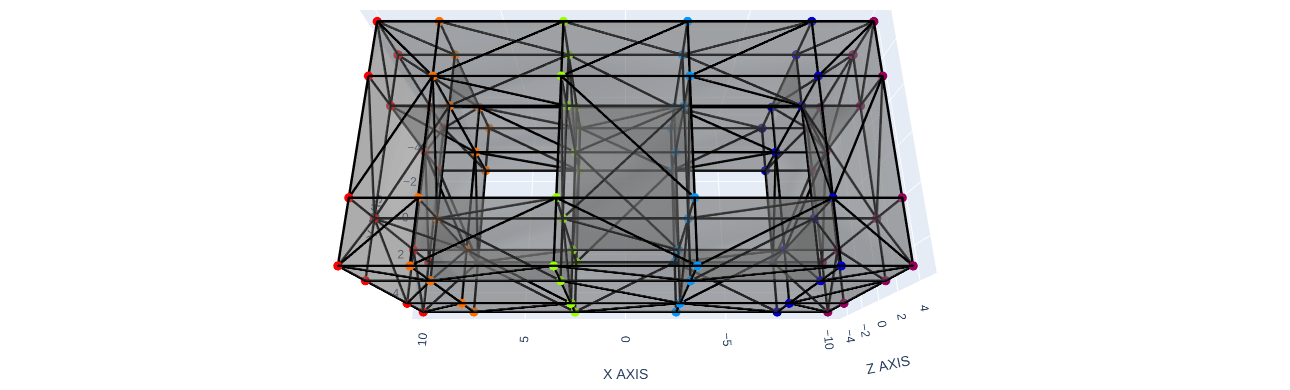
\includegraphics[width=3in]{Final Run, (two cubes, three pockets each, 00 mm apart) meshpy plotly screenshots.png}\\ {\fontsize{10}{12}\selectfont 00 mm apart}}  \\
    \bottomrule
    \end{tabular}
    \end{center}
    \caption{MeshPy Plots displayed with Plotly of two cubes with three CAD pocket operations that move closer together until combining.}
    \label{fig:cube_two_cubes_meshpy_table}
\end{table}

\begin{table}[H]
\begin{center}
    \begin{tabular}{cc}
         \includegraphics[width=1.875in]{Final Run, (two cubes, three pockets each, 50 mm apart) persdia.png} &
         \includegraphics[width=1.875in]{Final Run, (two cubes, three pockets each, 40 mm apart) persdia.png} \\ 
         \includegraphics[width=1.875in]{Final Run, (two cubes, three pockets each, 30 mm apart) persdia.png} &
         \includegraphics[width=1.875in]{Final Run, (two cubes, three pockets each, 20 mm apart) persdia.png} \\ 
         \includegraphics[width=1.875in]{Final Run, (two cubes, three pockets each, 10 mm apart) persdia.png} & 
         \includegraphics[width=1.875in]{Final Run, (two cubes, three pockets each, 00 mm apart) persdia.png} \\
\end{tabular}
\end{center}
    \caption{Persistence Diagrams of two cubes with three CAD pocket operations that move closer together until combining.}
    \label{fig:cube_two_cubes_persdia_table}
\end{table}

\chapter{Discussion}

%%------------------------------------------------------------------%%
%%------------------------ Bibliography ----------------------------%%
%%------------------------------------------------------------------%%
%% Replace the myreferences with the name of your bib file.  Then you
%% can run bibtex as usual.
%%------------------------------------------------------------------%%


\bibliography{thesis_bib}
\bibliographystyle{plain}

%%------------------------------------------------------------------%%
%%------------------------- Appendices -----------------------------%%
%%------------------------------------------------------------------%%
%% If you choose not to have appendices, comment out the \appendix
%% line and the chapters below.
%%------------------------------------------------------------------%%
\appendix
\chapter{Appendix}

%%------------------------------------------------------------------%%
\backmatter
%%------------------------------------------------------------------%%
%%----------------------- YOU ARE FINISHED ! -----------------------%%
%%------------------------------------------------------------------%%
\end{document}
